\documentclass[11pt]{article}

\usepackage{graphicx}
\usepackage{listings}
\usepackage{url}
\usepackage{float} % Add this package for the [H] option
\usepackage{listings}
\usepackage{color}

\definecolor{dkgreen}{rgb}{0,0.6,0}
\definecolor{gray}{rgb}{0.5,0.5,0.5}
\definecolor{mauve}{rgb}{0.58,0,0.82}
\usepackage{minted}

\lstset{frame=tb,
  language=Java,
  aboveskip=3mm,
  belowskip=3mm,
  showstringspaces=false,
  columns=flexible,
  basicstyle={\small\ttfamily},
  numbers=none,
  numberstyle=\tiny\color{gray},
  keywordstyle=\color{blue},
  commentstyle=\color{dkgreen},
  stringstyle=\color{mauve},
  breaklines=true,
  breakatwhitespace=true,
  tabsize=3
}

\begin{document}

\begin{titlepage}
    \begin{center}
        
\includegraphics[scale=0.10]{du.png}\par
        \begin{Huge}
            \textsc{University of Dhaka}\par
        \end{Huge}
        \begin{Large}
            Department of Computer Science and Engineering\par \vspace{1cm}
            CSE-3111 : Computer Networking Lab \\[12pt]   
            Lab Report 2 : Introduction to Client-Server \\[5pt]Communication using Socket Programming — Simulating \\[5pt]an ATM Machine Operation
        \end{Large}
    \end{center}     
    \begin{large}
        \textbf{Submitted By:\\[12pt]}
            Name: Md Shamsur Rahman Sami\\[5pt]
            Roll No : 57\\[7pt]
            Name: Md Rakib Hossain\\[5pt]
            Roll No : 55\\[12pt]
        \textbf{Submitted On : \\[12pt]}
            January 26, 2024\\[20pt]
        \textbf{Submitted To :\\[12pt]}
            Dr. Md. Abdur Razzaque\\[12pt]
    \end{large}
\end{titlepage}

\tableofcontents  

\newpage

\section{Introduction}
\subsection{Objectives}

\section*{Creating TCP Connections using Socket Programming}

\begin{itemize}
  \item Socket programming can be used to establish a TCP connection between a client process running on host B and a server process running on host A.
  
  \begin{itemize}
    \item For a line of text, the client process can send a request including a tiny letter to the server process, which will then transform all small letters to capital letters and return the modified text back to the client process.
    
    \item Finding out if a number is palindrome or not: The client process can send a request including a number to the server process, which will determine if the number is palindrome or not and reply to the client process with the outcome.
  \end{itemize}

  \item It is possible to implement a non-idempotent operation utilizing exactly-once semantics to handle failures of request and response messages as well as failures of process execution.
  
  \begin{itemize}
    \item  It is possible to create an application-level protocol that enables the verification of a user's card and password, the checking of their account balance, and the making of account withdrawals. Messages like: 
    
    \begin{itemize}
      \item Request for verification of card , password
      \item Request for user account balance
      \item Request for user withdrawal
      \item Confirmation of user withdrawal
      \item Error message if there is not enough money in the account of user 
    \end{itemize}

    \item To handle errors related to both request and response messages, the protocol can include a mechanism for resending messages in case of failures and an acknowledgment system to confirm.
  \end{itemize}
\end{itemize}

\section{Theory}
Socket programming is a method of inter-process communication (IPC) that
allows processes to communicate with each other across a network using
sockets. A socket is a endpoint for sending or receiving data across a computer network. It is a combination of an IP address and a port number.
In socket programming, a client creates a socket and connects to a server
using the server’s IP address and port number. The server then creates a
socket and binds it to a specific IP address and port number. Once the
connection is established, the client and server can send and receive data
through the socket.
\subsection{Server}
When we started server side program , it will wait for client requests. If it
gets any request then it will establish a connection.

\subsection{Client}
From client side , We will enter IP address of our server and
the port number. Then the client connection request will be sent from our
client to the server.



\section{Methodology}

Socket programming allows the creation of TCP (Transmission Control Protocol) connections through a series of phases that include socket creation, server connection, and data sending and receiving. It gets an HTTP query indicating the file the client requested after establishing the connection. After that, it will send the client the bytes it read from that file.

\subsection{Creating a Socket}

First we create a socket using the \texttt{socket()} function. This function takes three parameters: the address family, the type of socket, and the protocol.

\subsection{Connecting to a Server}

After creating the socket is created, the next step is to connect to a server using the \texttt{connect()} function. This function takes three parameters: the socket descriptor, the server's IP address, and the server's port number.

\subsection{Sending and Receiving Data}

Once the connection is established, the client and server can send and receive data through the socket.

\subsection{Closing the Connection}

When data exchange is complete, the connection can be closed using the \texttt{close()} function. This function takes one argument: the socket descriptor.

\subsection{Idempotent Operation}

In computing, an idempotent operation is one that has no additional effect if it is called more than once with the same input parameters. For example, removing an item from a set can be considered an idempotent operation on the set.

\subsection{Exactly-once Semantics}

As its name suggests, exactly-once semantics means that each message is delivered precisely once. The message can neither be lost nor delivered twice (or more times). Exactly-once is by far the most dependable message delivery guarantee.




\section{Experimental Result}

\subsection{Establish a TCP connection in between a server process, running on host A and a client process,running on host B and then perform some operation by the server process requested by theclient and send responses from the server.}


\begin{itemize}
    \item \textbf{Small Letter to Capital Conversion for a Line of Text:}
    
    Here first we create a connection with client and server and than send a small letter text from client to the server , server accept the client request and convert it into big letter and send the response to the client . 
    \begin{minted}[mathescape, linenos]{python}
    SERVER SIDE CODE
   
import socket

s = socket.socket(socket.AF_INET, socket.SOCK_STREAM)
s.bind((socket.gethostname(), 1234))
s.listen(5)
print(socket.gethostname())

while True:
    try:
        clientsocket, address = s.accept()
        print(f"Connection from {address} has been established")
       # clientsocket.send(bytes("Welcome ", "utf-8"))
        msgg= clientsocket.recv(1024)
        sami=msgg.decode("utf-7")
        samiii =sami.lower()
        print("I am receiving the message form client= " +sami)
        clientsocket.send(bytes(samiii, "utf-8"))

        print(sami)
        
    except Exception as e:
        print(f"Error: {e}")


    clientsocket.close()
\end{minted}


    \begin{minted}[mathescape, linenos]{python}
    CLIENT SIDE CODE
import socket

#socket first
s=socket.socket(socket.AF_INET,socket.SOCK_STREAM)
s.connect(("192.168.0.6", 5000))
message = "HELLO SERVER"
s.send(message.encode('utf-7'))

msg= s.recv(1024)
print("Sending  data from client :"+ message)

print("After receiving Data Fron Server : "+msg.decode("utf-8"))
s.close()
\end{minted}
    \begin{figure}[H]
        \centering
        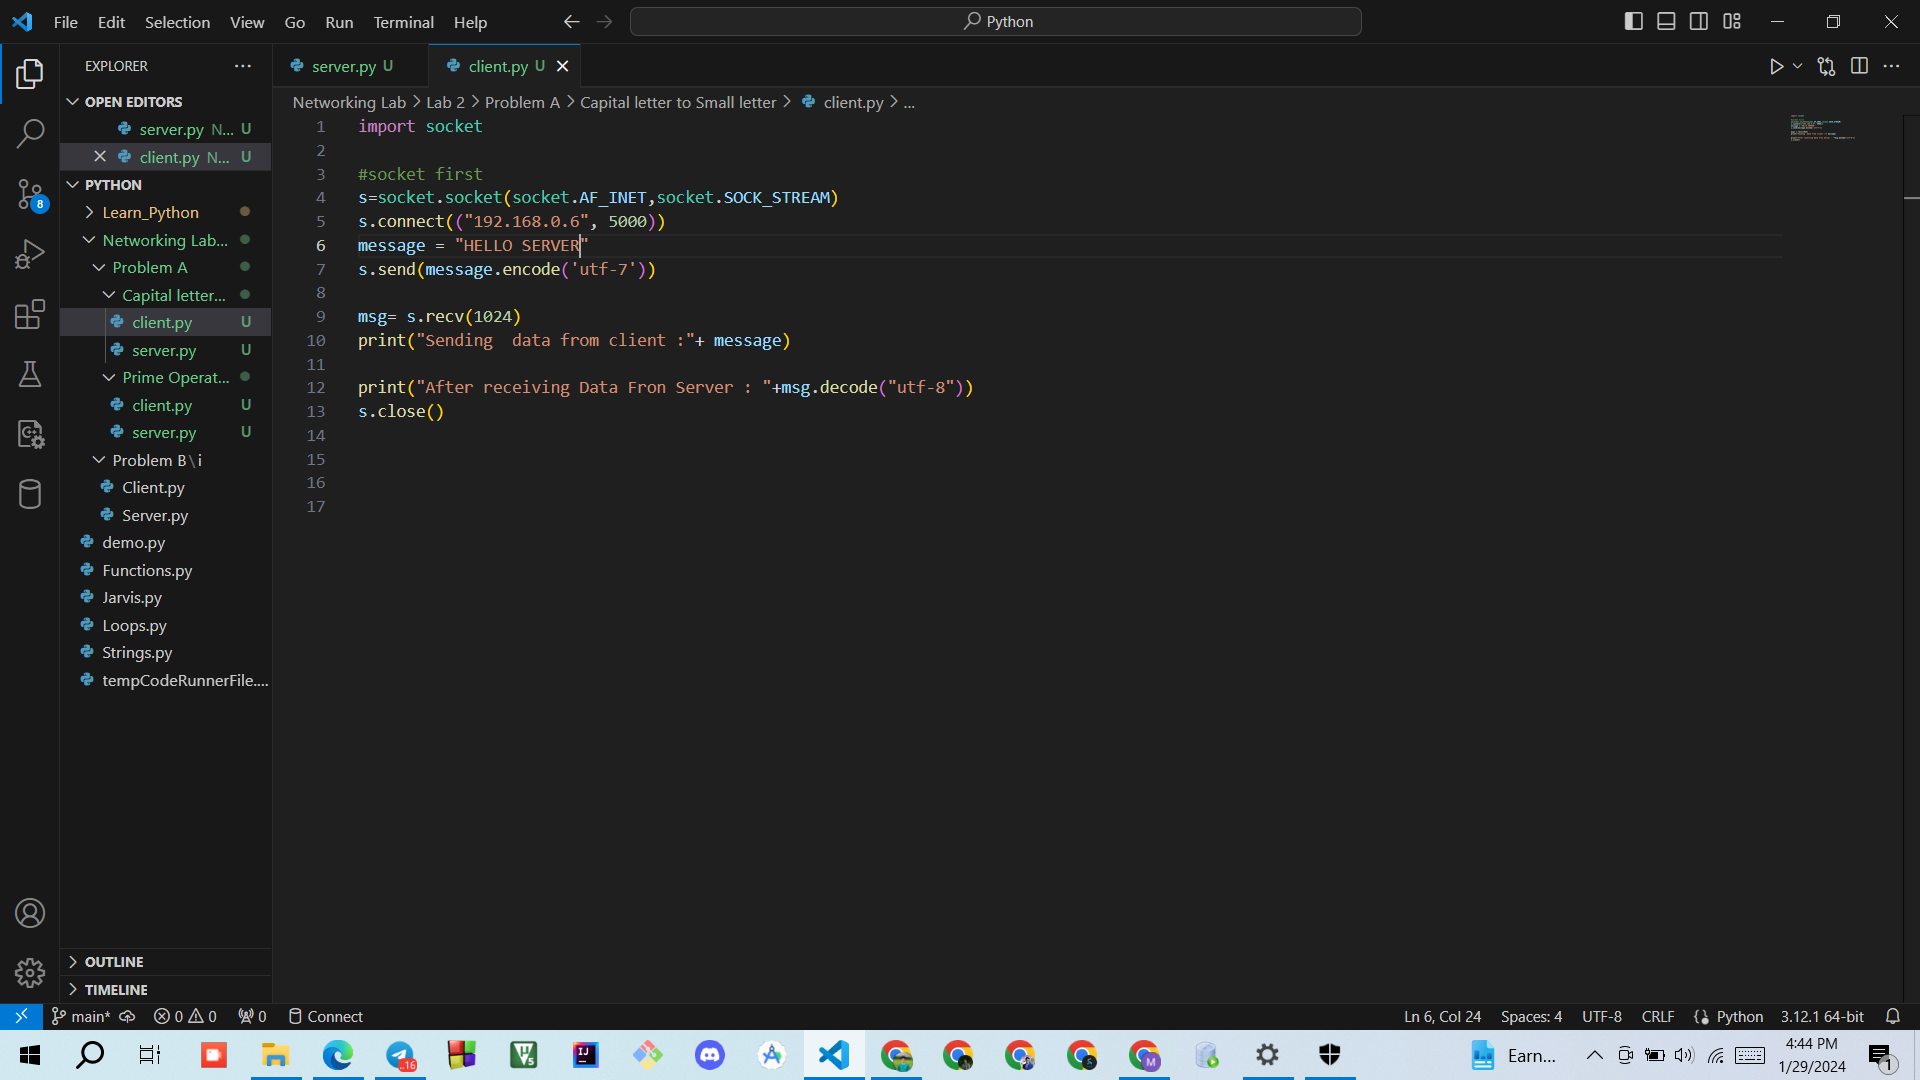
\includegraphics[width=0.8\textwidth]{small.client.png}
        \caption{Client side code}
        \label{fig:1}
    \end{figure}
    
    \begin{figure}[H]
        \centering
        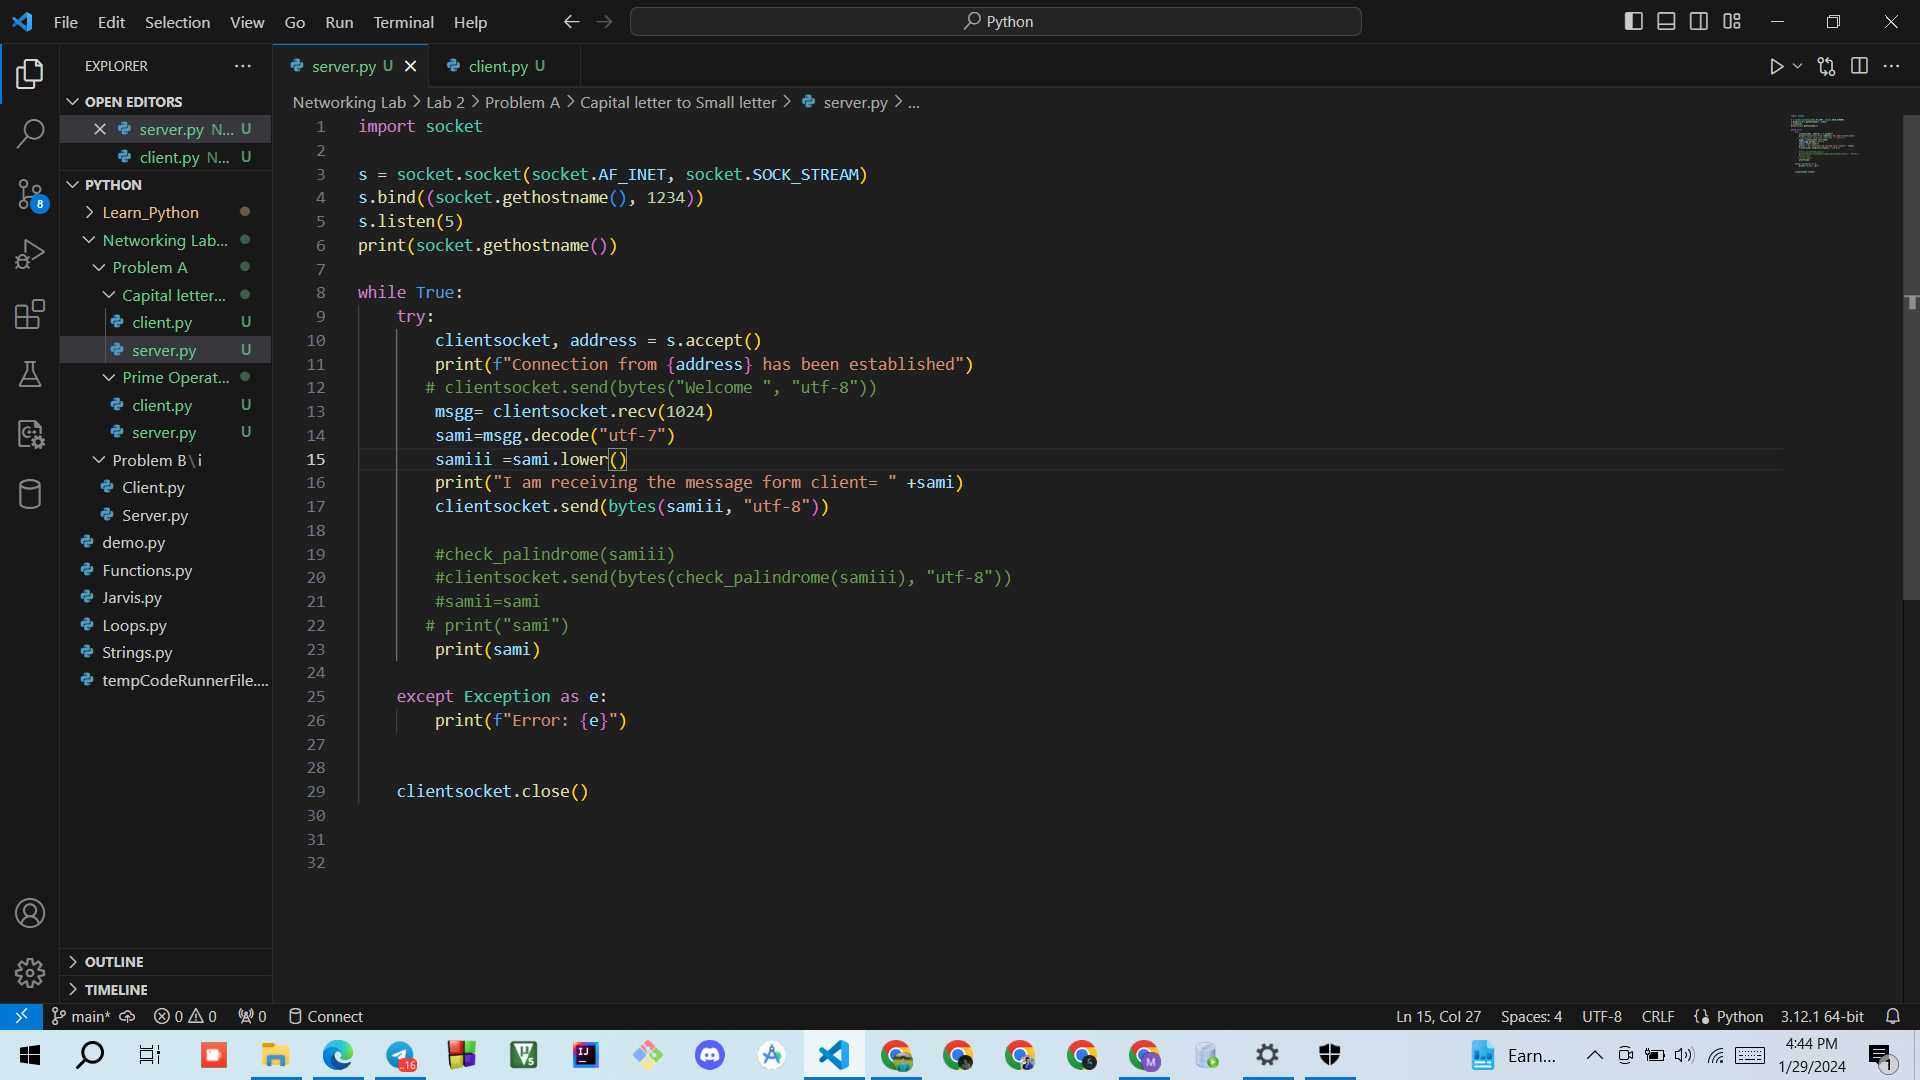
\includegraphics[width=0.8\textwidth]{small.server.png}
        \caption{Server Side Code}
        \label{fig:2}
    \end{figure}
    
    \begin{figure}[H]
      \centering
      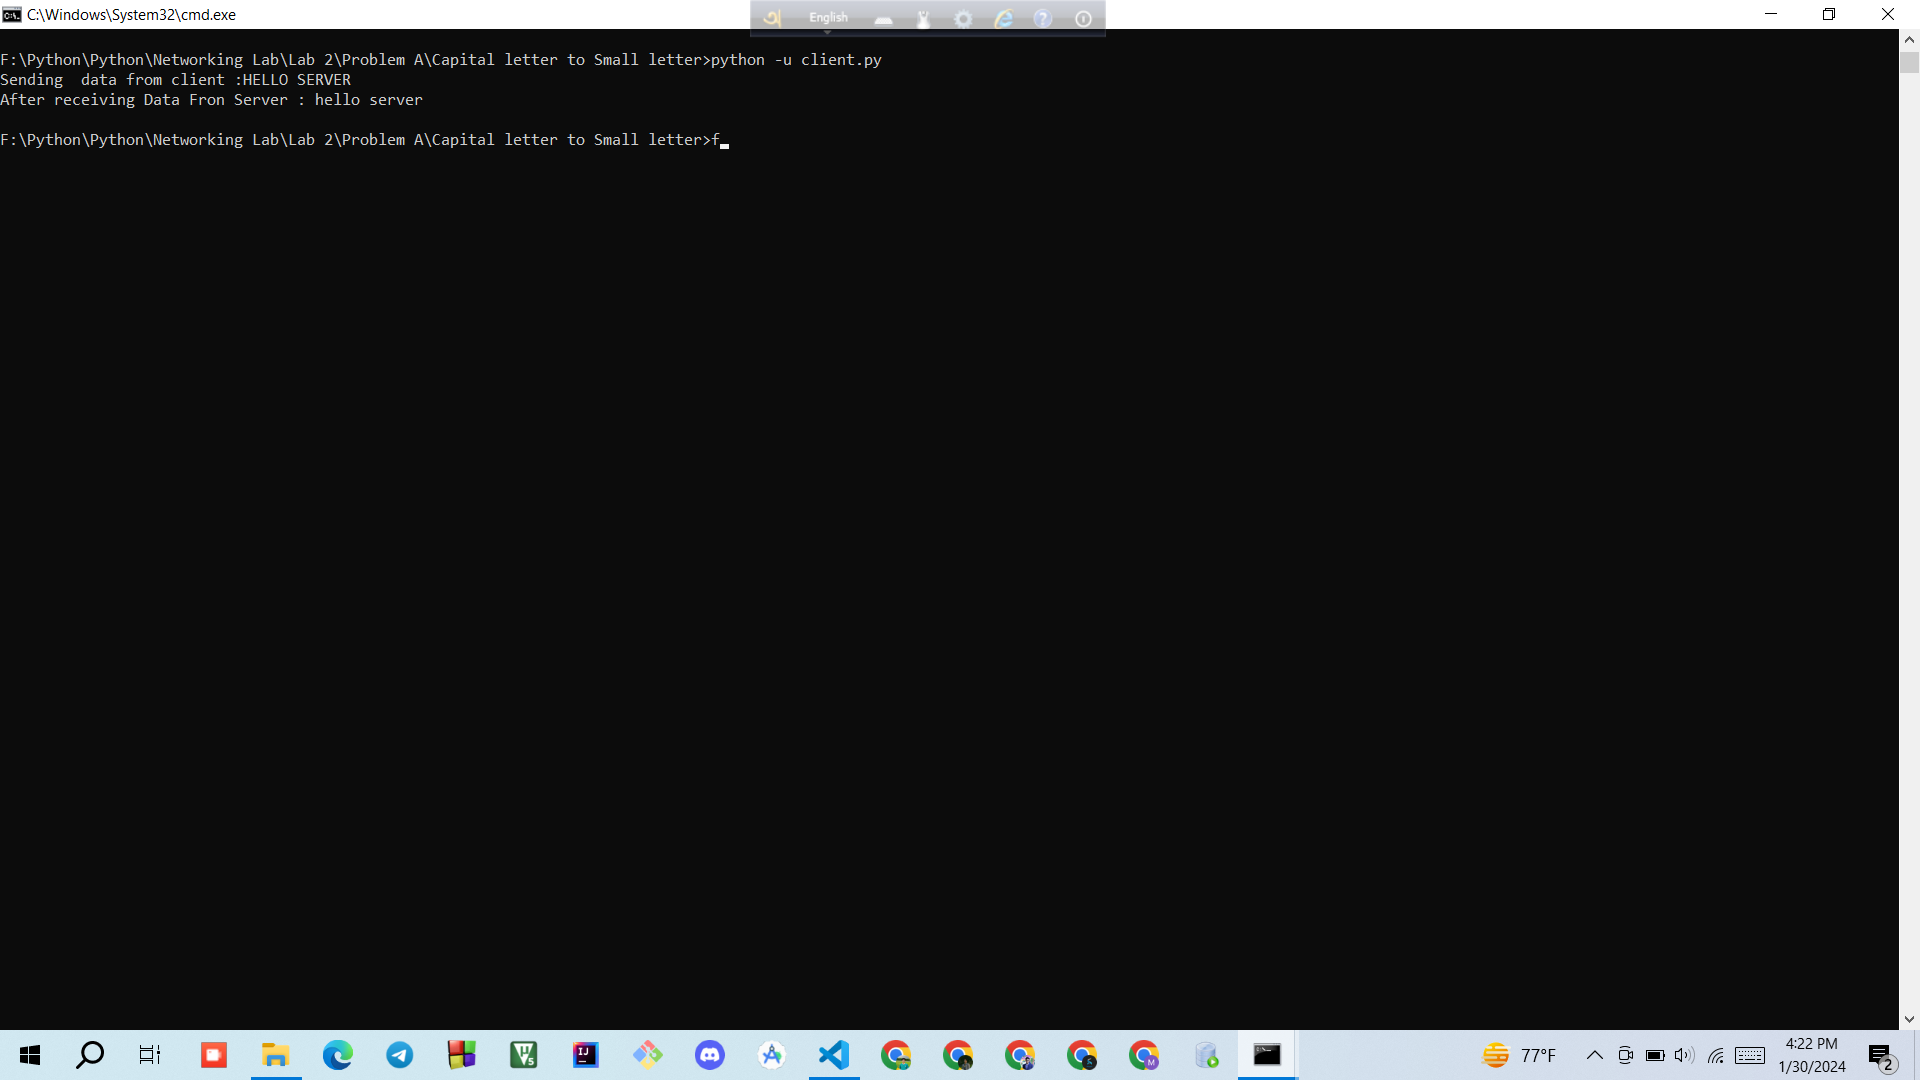
\includegraphics[width=0.8\textwidth]{small_result.client.png}
      \caption{Client Side result}
      \label{fig:3}
    \end{figure}
    
    \begin{figure}[H]
      \centering
      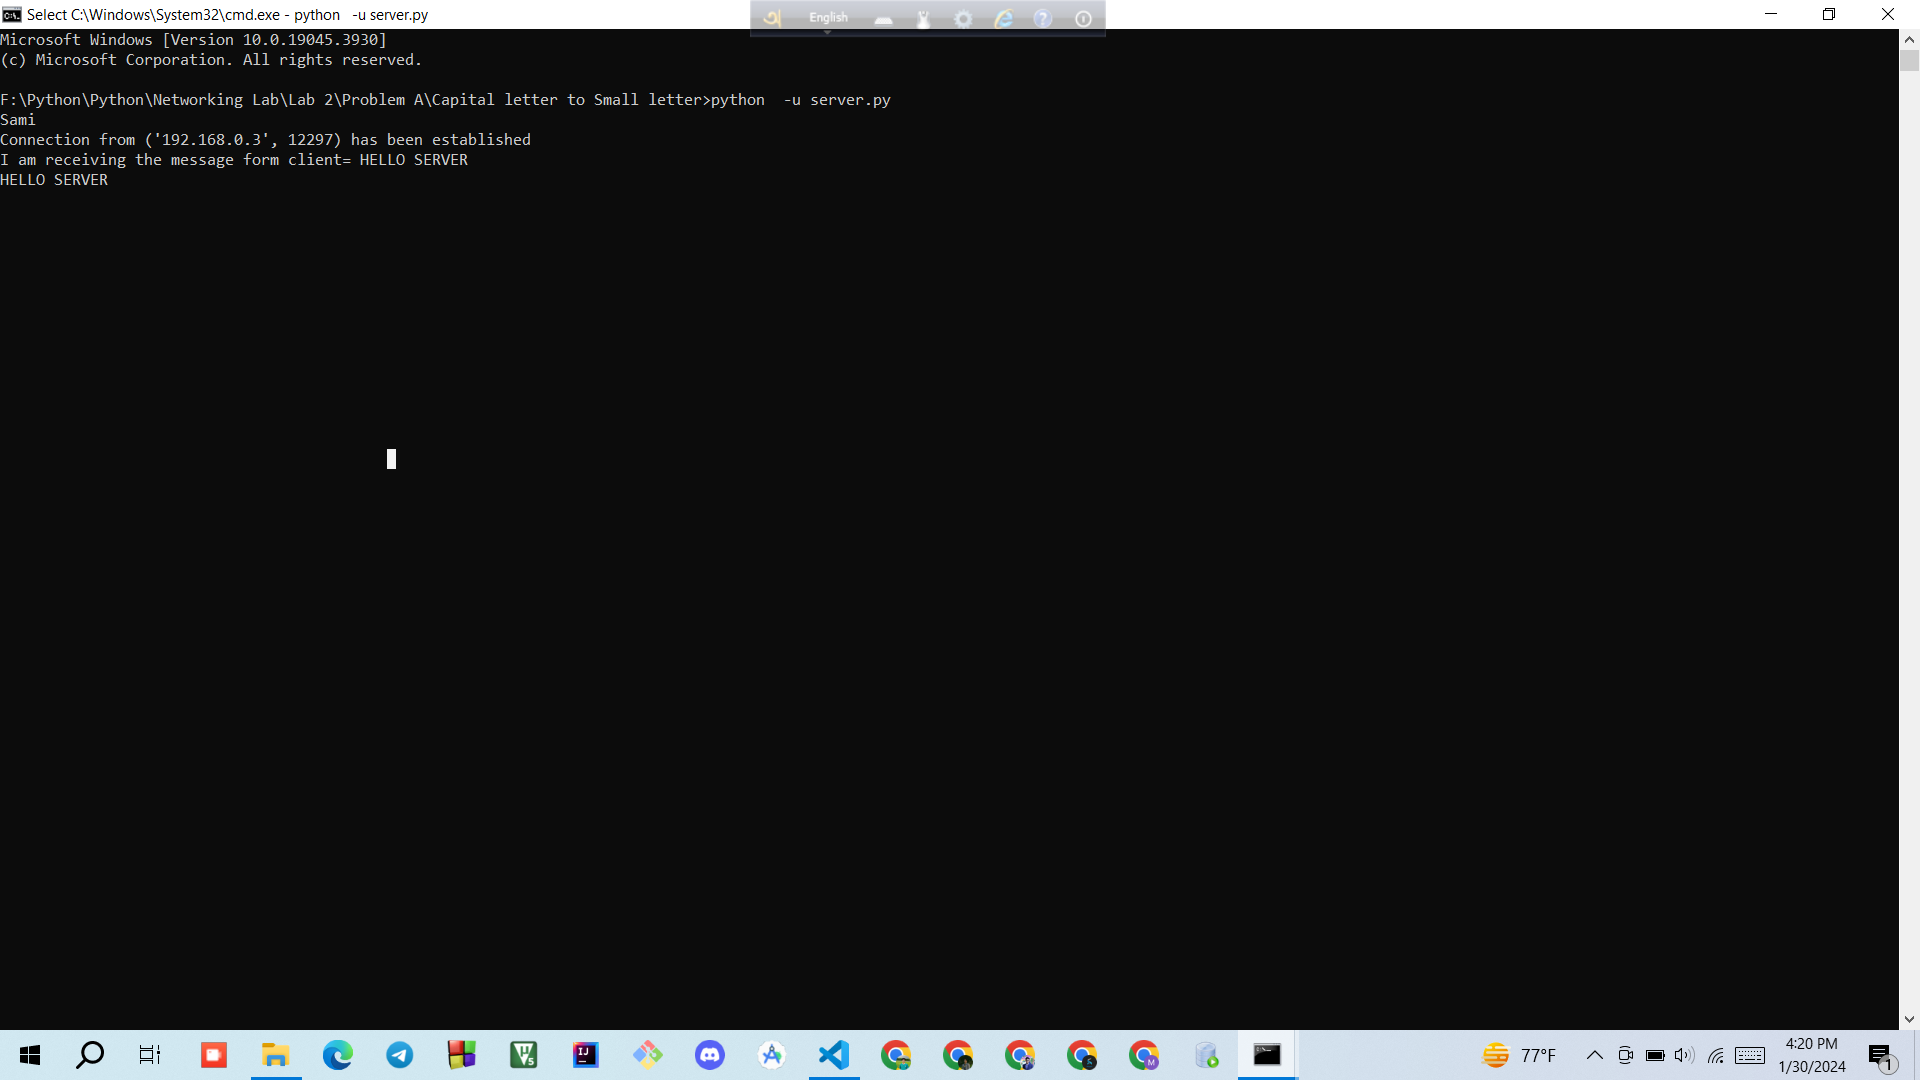
\includegraphics[width=0.8\textwidth]{small_result.server.png}
      \caption{Server Side result}
      \label{fig:4}
    \end{figure}

\end{itemize}

 
\subsection{Send an integer and operation name (either ‘prime’ or ‘palindrome’) to the server and check whether it’s a prime (or palindrome) or not.}
    \begin{minted}[mathescape, linenos]{python}
    SERVER SIDE CODE
    import socket

def is_prime(n):
    if n <= 1:
        return False
    elif n <= 3:
        return True
    elif n % 2 == 0 or n % 3 == 0:
        return False
    i = 5
    while i * i <= n:
        if n % i == 0 or n % (i + 2) == 0:
            return False
        i += 6
    return True

s = socket.socket(socket.AF_INET, socket.SOCK_STREAM)
s.bind((socket.gethostname(), 1234))
s.listen(5)

while True:
    connection, address = s.accept()
    print(f"Connection from {address} has been established")
    try:
        data = connection.recv(1024)
        data = int(data.decode())
        success = is_prime(data)
        if success:
            connection.sendall("It is a prime number".encode())
        else:
            connection.sendall("It is not a prime number".encode())
    finally:
        connection.close()

\end{minted}
    \begin{minted}[mathescape, linenos]{python}
    CLIENT SIDE CODE
   import socket

s = socket.socket(socket.AF_INET, socket.SOCK_STREAM)

s.connect(("Sami", 1234))

try:
    request = int(input("Enter a number: "))

    s.sendall(str(request).encode())
    response = s.recv(1024).decode()
    print("The number is ",request," "+response)

finally:
    s.close()
\end{minted}

\begin{itemize}
    \item \textbf{}
    
  . 
    \begin{figure}[H]
        \centering
        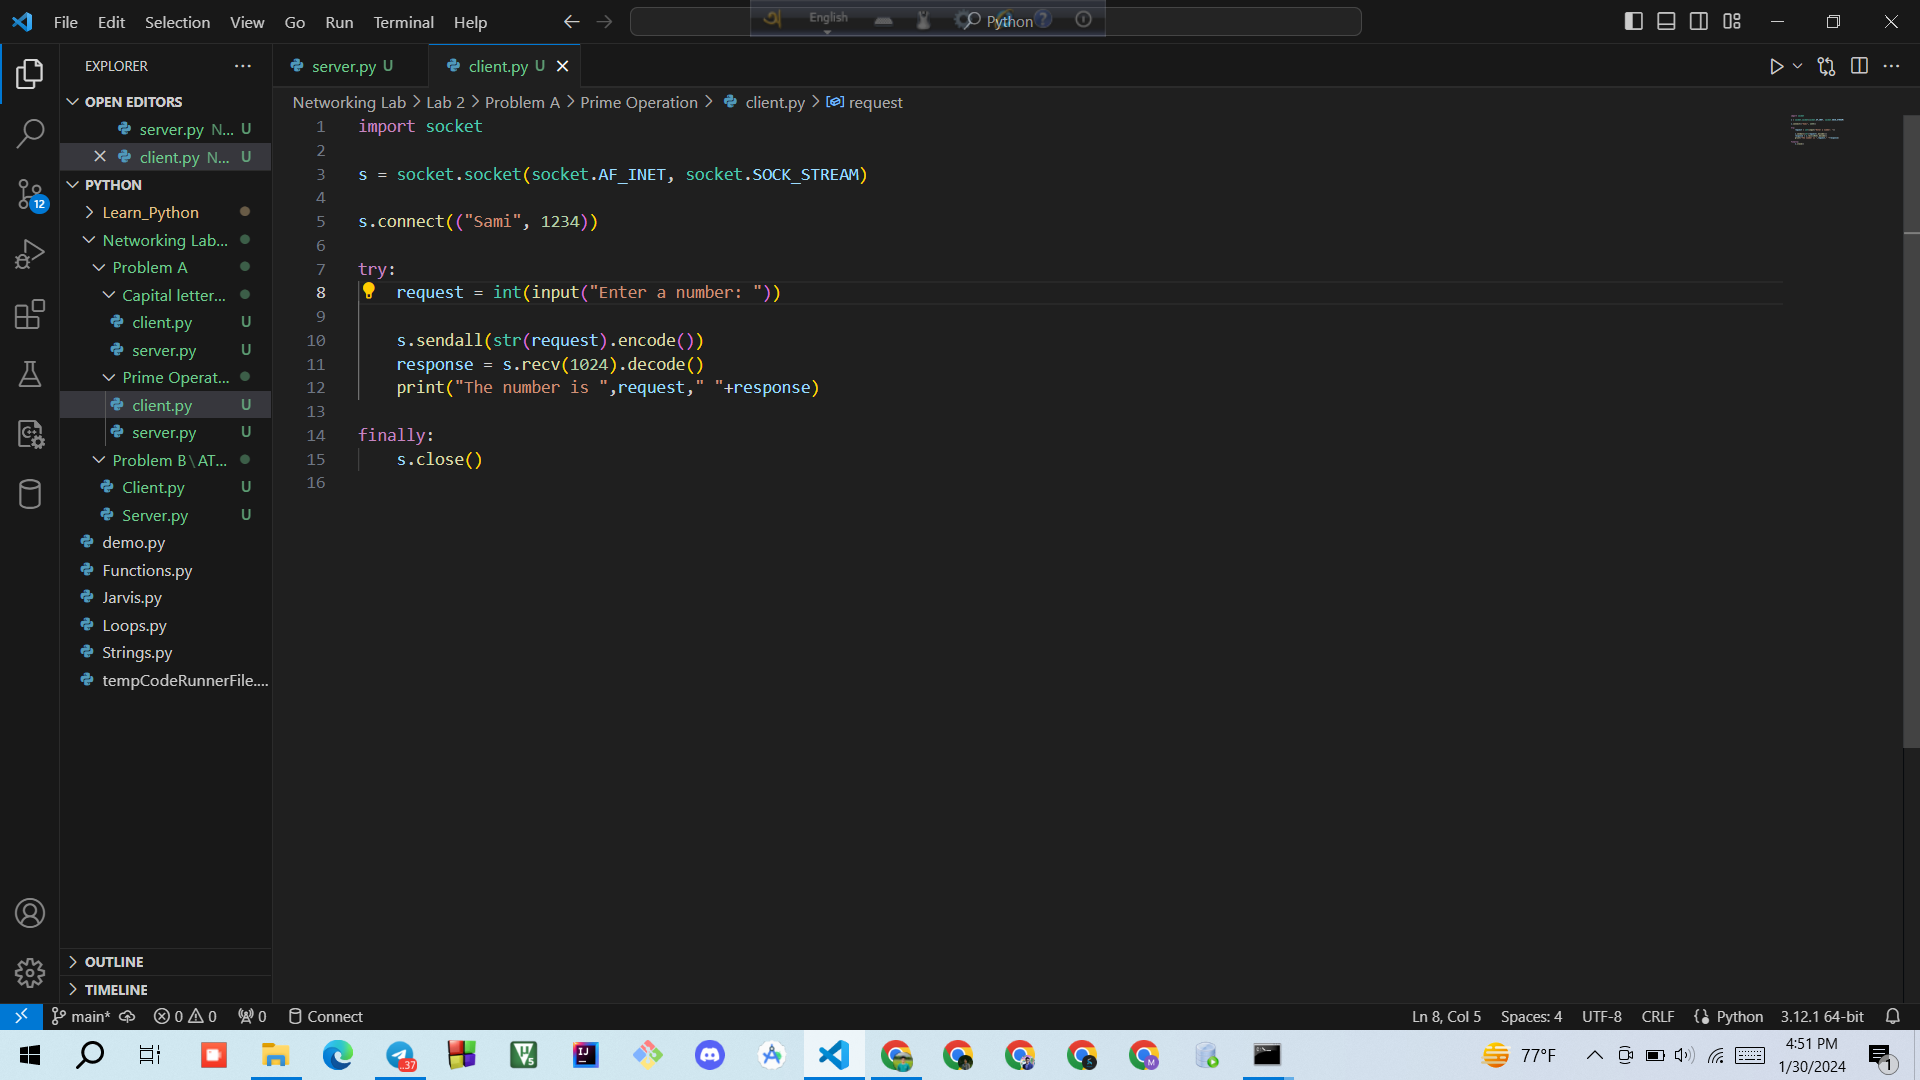
\includegraphics[width=0.8\textwidth]{prime.client.png}
        \caption{Client side code}
        \label{fig:1}
    \end{figure}
    
    \begin{figure}[H]
        \centering
        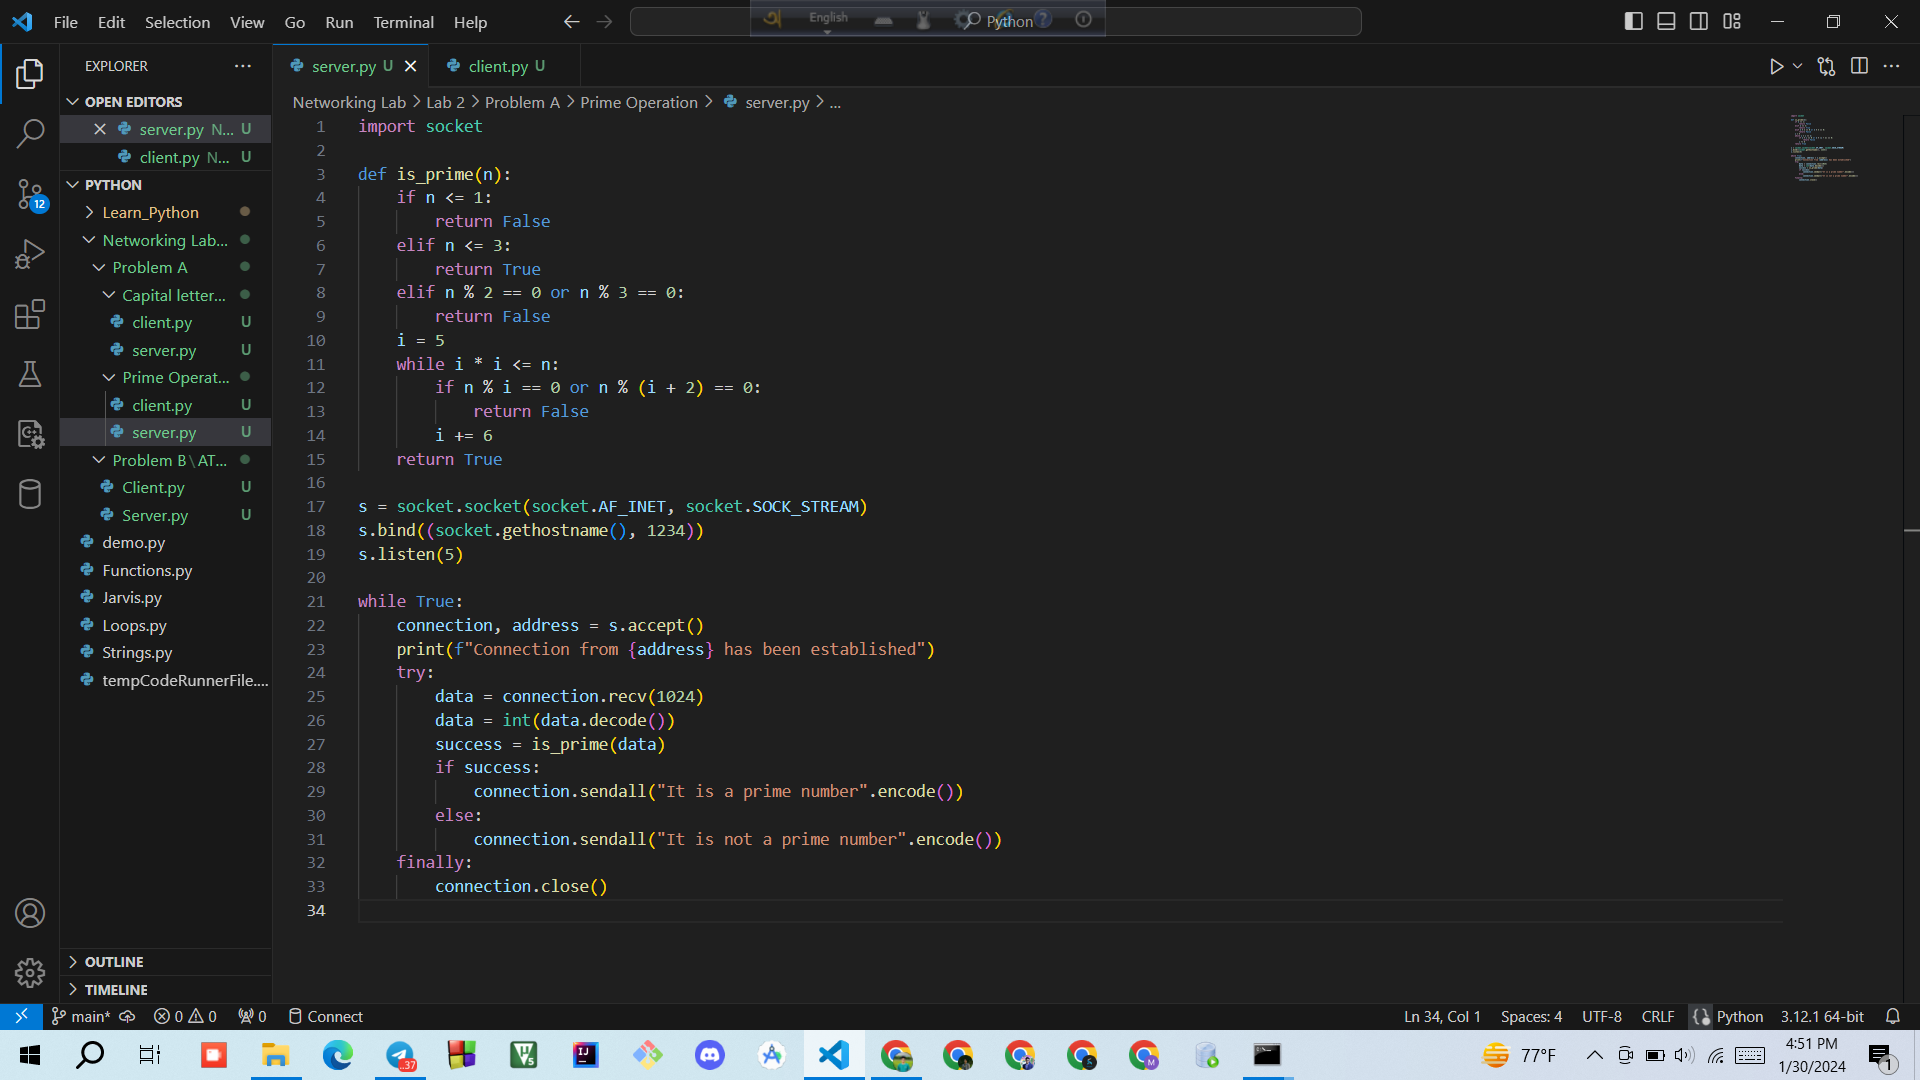
\includegraphics[width=0.8\textwidth]{prime.server.png}
        \caption{Server Side Code}
        \label{fig:2}
    \end{figure}
    
    \begin{figure}[H]
      \centering
      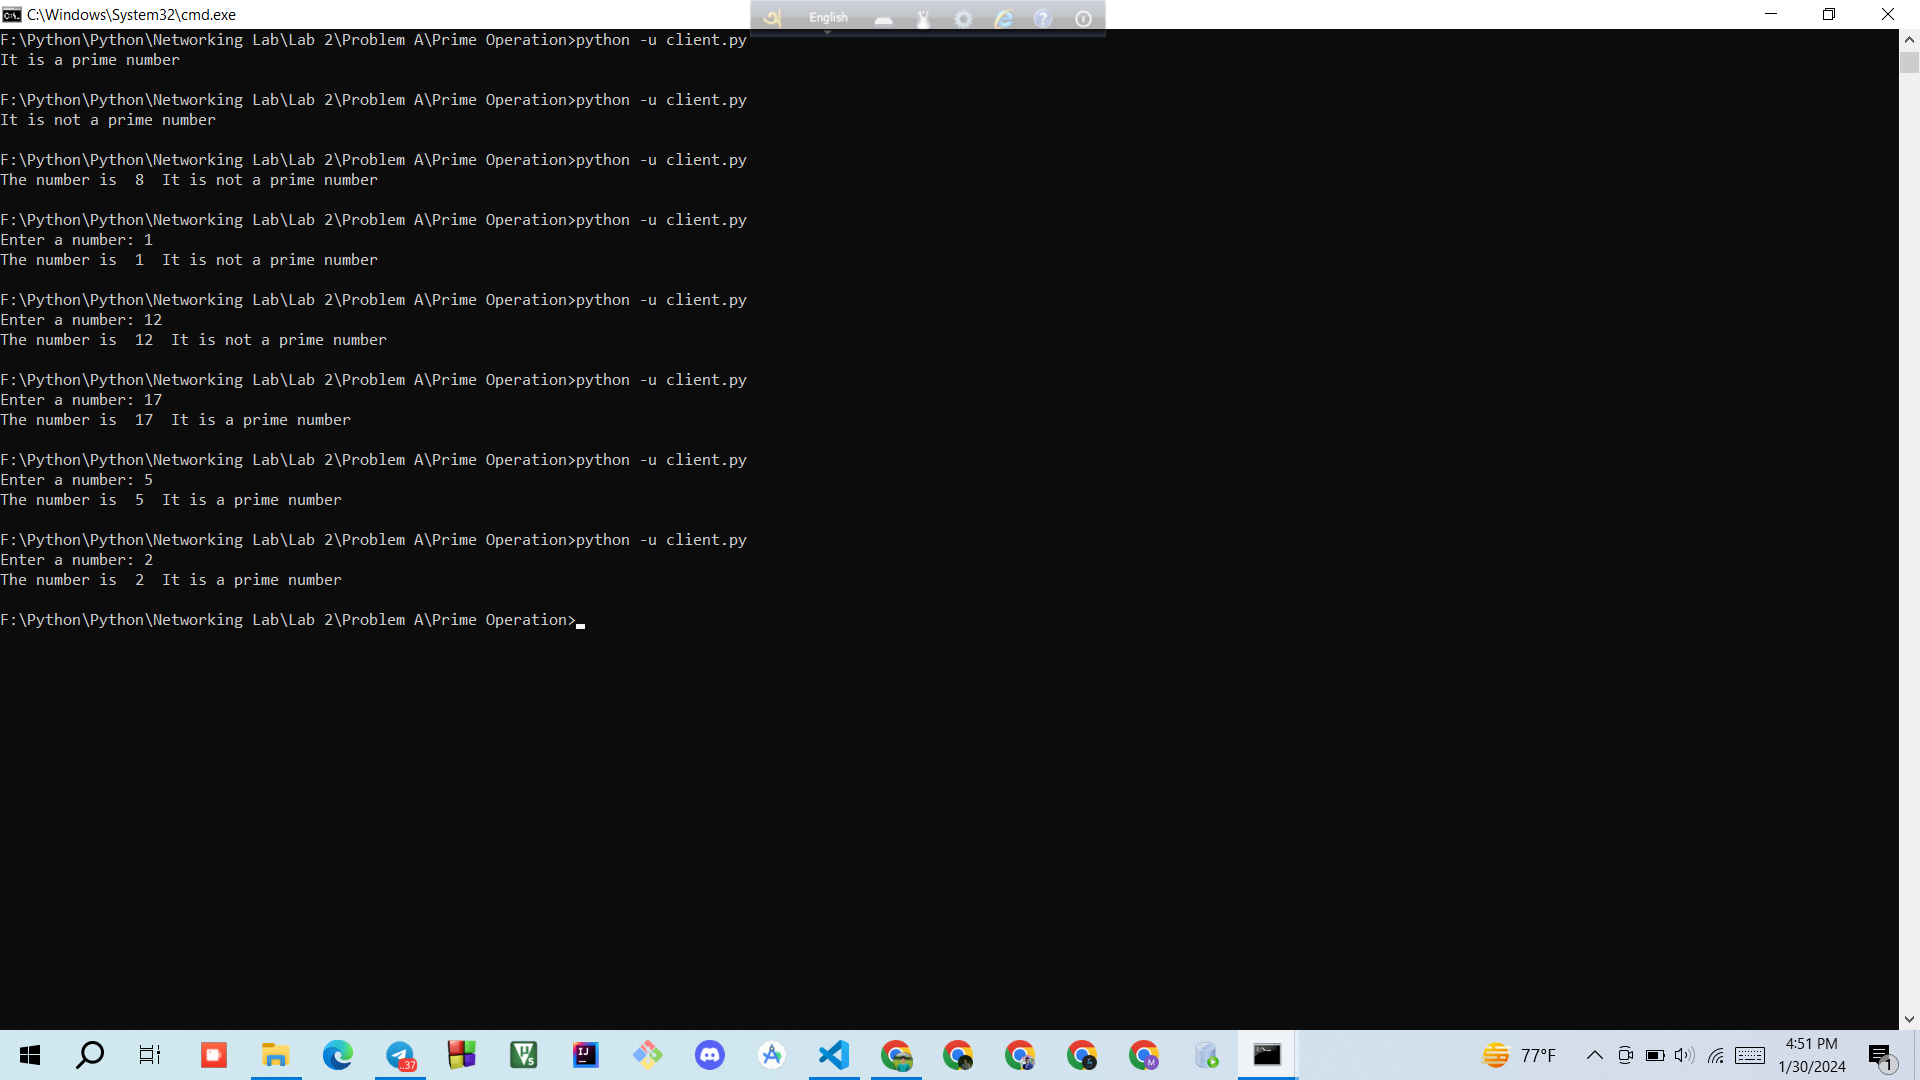
\includegraphics[width=0.8\textwidth]{prime_result.client.png}
      \caption{Client Side result}
      \label{fig:3}
    \end{figure}
    
    \begin{figure}[H]
      \centering
      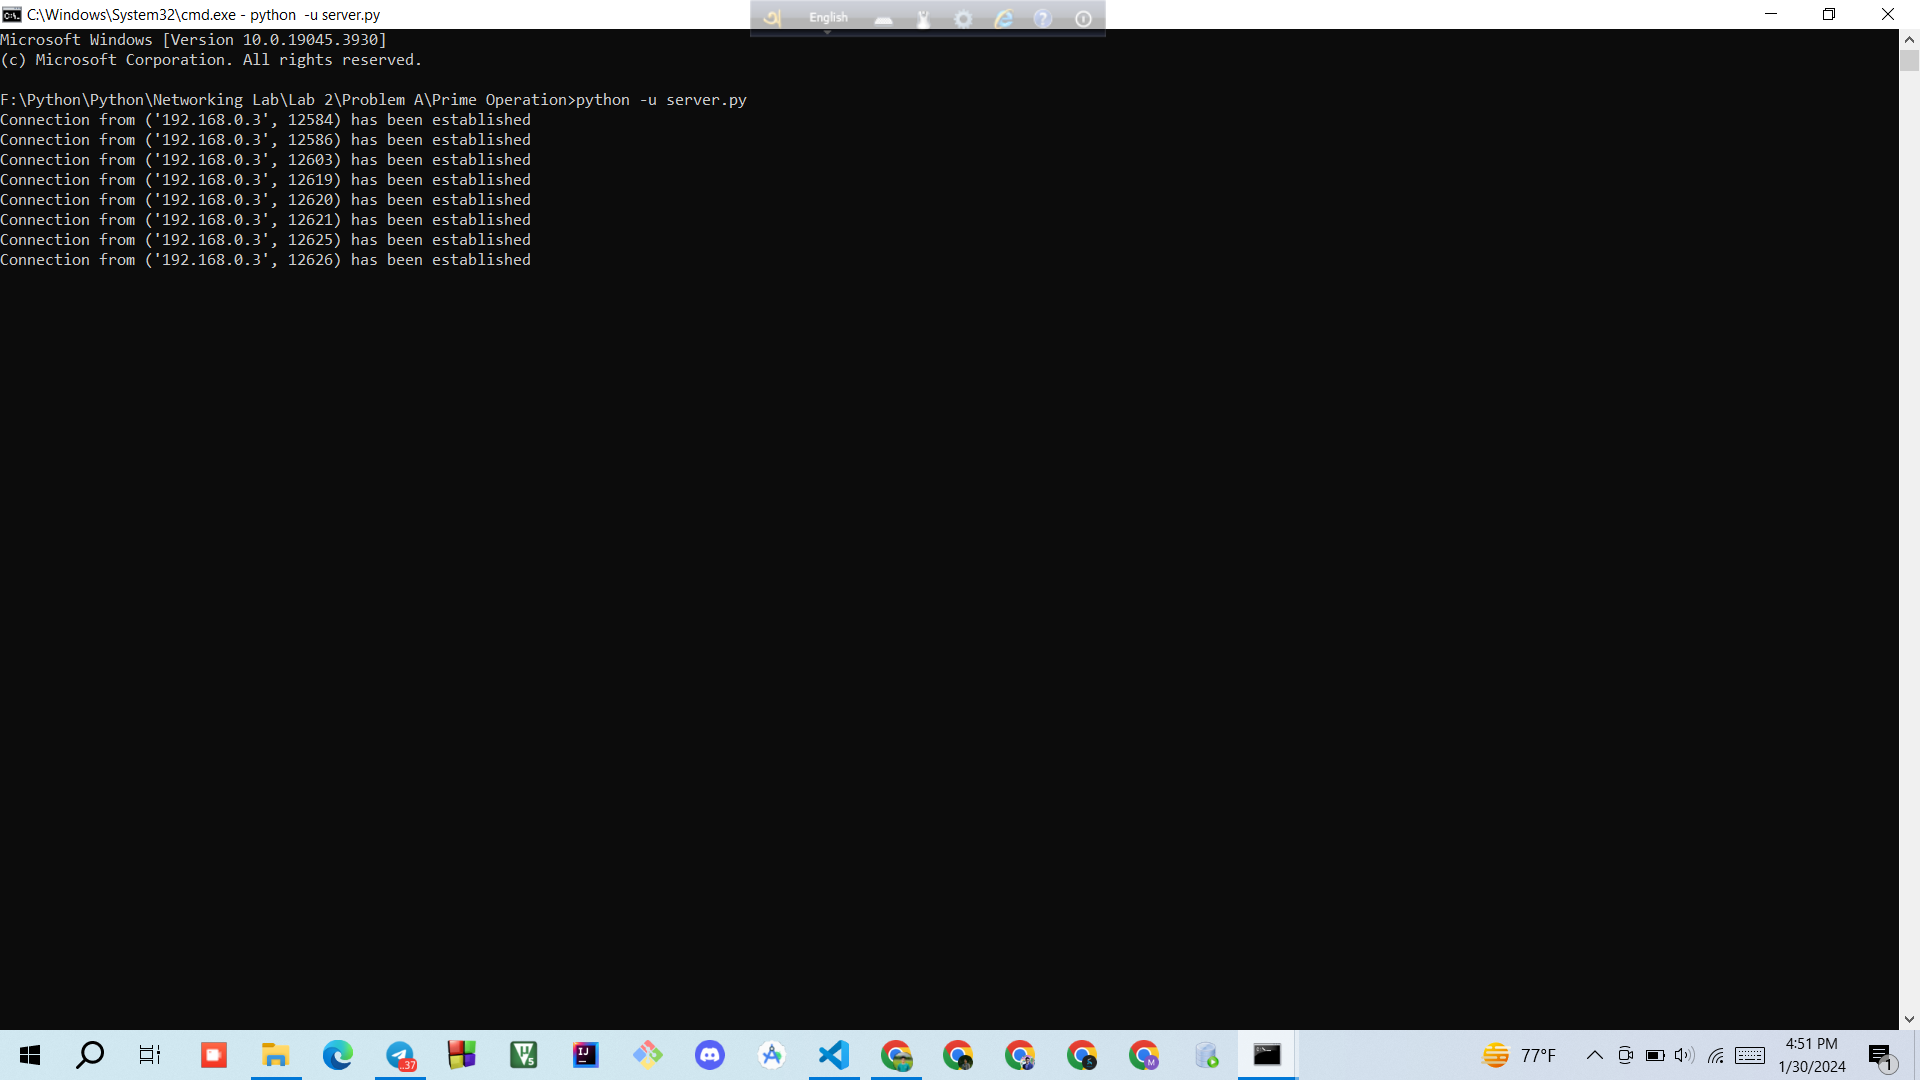
\includegraphics[width=0.8\textwidth]{prime_result.server.png}
      \caption{Server Side result}
      \label{fig:4}
    \end{figure}

\end{itemize}




\subsection{Using the above connection, design and implement a non-idempotent operation using exactly-once semantics that can handle the failure of request messages, failure of response messages
and process execution failures.}


\begin{itemize}
    \item \textbf{Enhance the above protocol so that it can handle errors related to both
request and response messages to and from the server.}
\begin{minted}[mathescape, linenos]{python}
    SERVER SIDE CODE
    import socket


accounts = {
    "123456789": {"password": "1234", "balance": 1000}
}

def process_withdrawal(card_number, password, amount):
    if card_number in accounts and accounts[card_number]["password"] == password:
        if accounts[card_number]["balance"] >= amount:
            accounts[card_number]["balance"] -= amount
            return True, accounts[card_number]["balance"]
        else:
            return False, "Insufficient funds"
    else:
        return False, "Invalid card number or password"




s=socket.socket(socket.AF_INET,socket.SOCK_STREAM)
s.bind((socket.gethostname(),1234))
s.listen(5)


while True:
    connection,address = s.accept()
    print(f"Connection from {address} has been established")

    try:
        
        # Receive the data from the ATM
        data = connection.recv(1024)
        data = data.decode().split(',')

        if len(data) == 4:
            # Process the received data
            card_number, password, operation, amount = data

            if operation == "WITHDRAW":
                success, response = process_withdrawal(card_number, password, int(amount))
                if success:
                    # Send success response to ATM
                    connection.sendall(f"SUCCESS,{response}".encode())
                else:
                    # Send failure response to ATM
                    connection.sendall(f"FAILURE,{response}".encode())
            else:
                connection.sendall("FAILURE,Invalid operation".encode())
        else:
            connection.sendall("FAILURE,Invalid request format".encode())

    finally:
        # Clean up the connection
        connection.close()
\end{minted}

    \begin{minted}[mathescape, linenos]{python}
    Client Side Code
   import socket

# Function to perform withdrawal
def withdraw(client_socket, card_number, password, amount):
    request = f"{card_number},{password},WITHDRAW,{amount}"
    client_socket.sendall(request.encode())
    response = client_socket.recv(1024).decode()
    return response.split(',')

# Create a TCP/IP socket
client_socket = socket.socket(socket.AF_INET, socket.SOCK_STREAM)

client_socket.connect((socket.gethostname(), 1234))
print(socket.gethostname())

try:
    # Example withdrawal request
    card_number = "123456789"
    password = "1234"
    amount = 500

    # Send withdrawal request to the server
    response_code, message = withdraw(client_socket, card_number, password, amount)

    # Process the response
    if response_code == "SUCCESS":
        print(f"Withdrawal successful. Updated balance: {message}")
    else:
        print(f"Withdrawal failed: {message}")

finally:
    # Clean up the connection
    client_socket.close()
\end{minted}
  
   
    \begin{figure}[H]
        \centering
        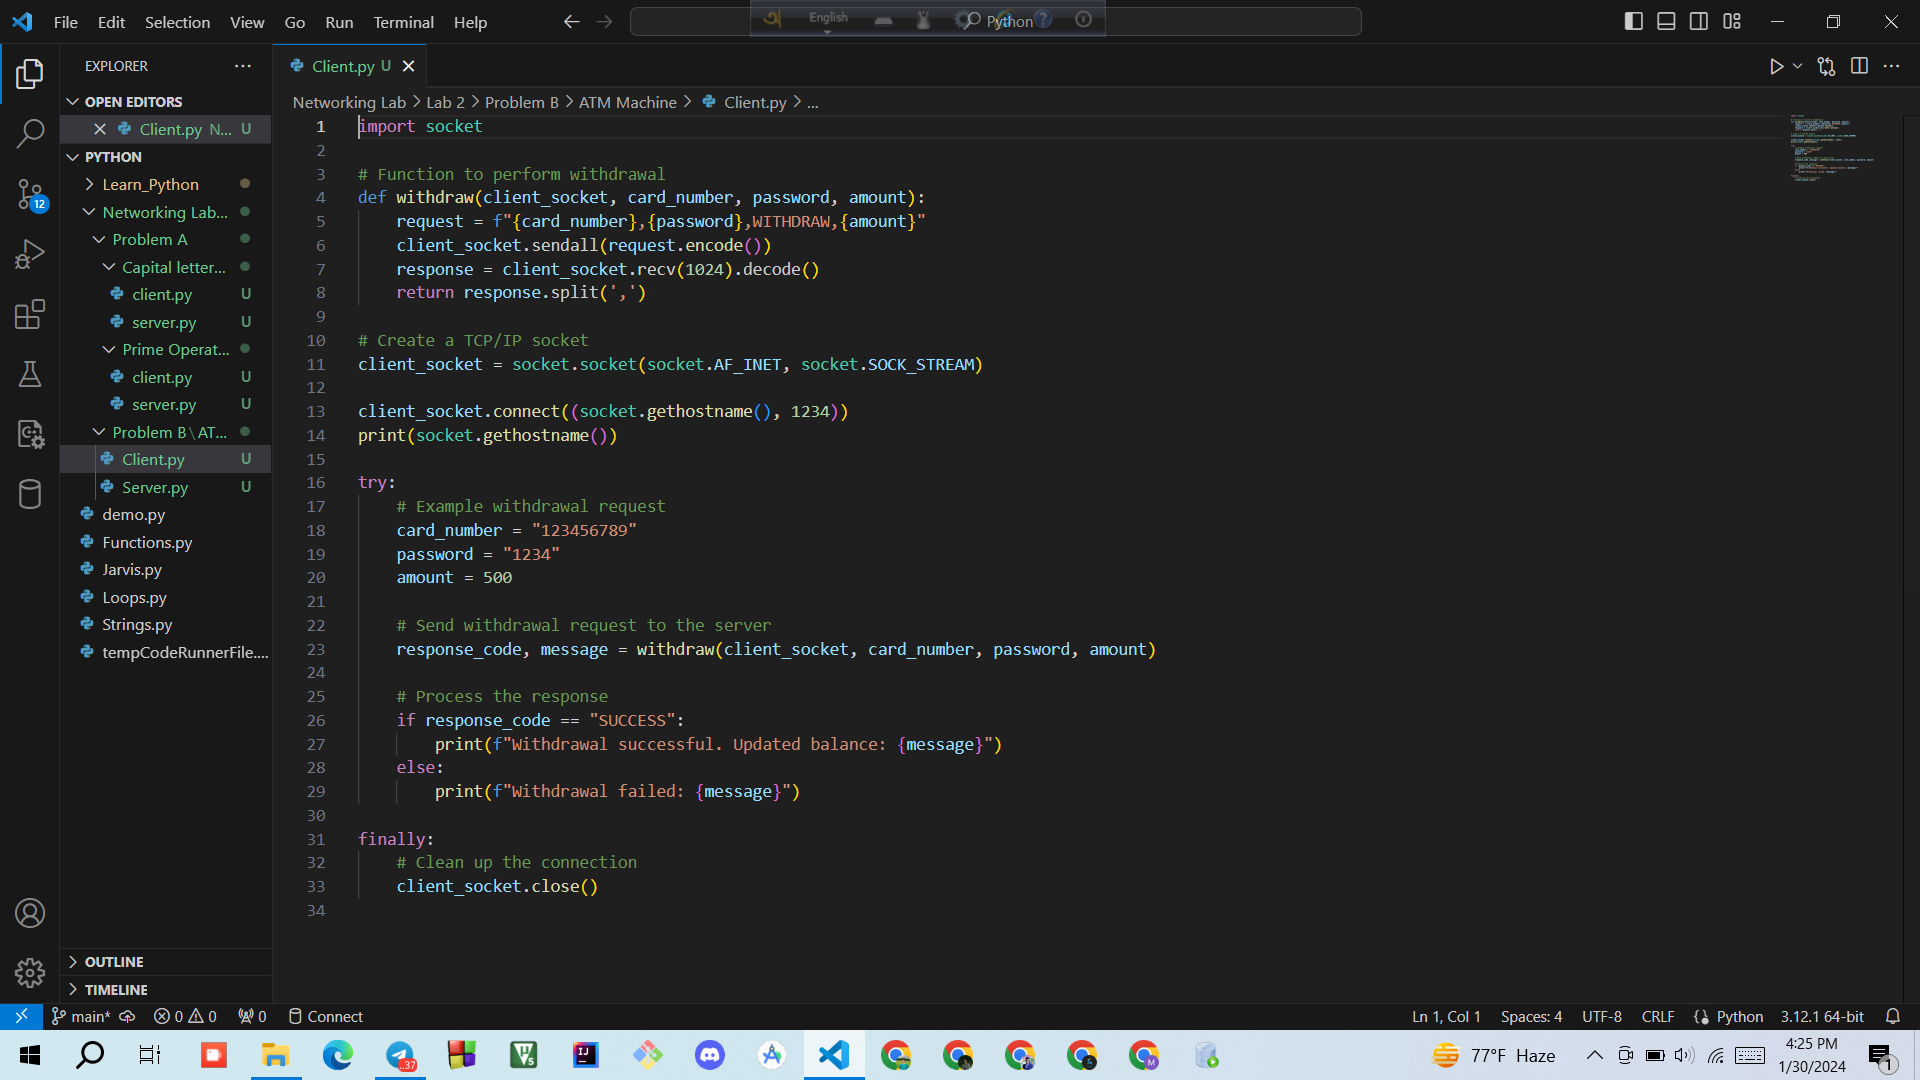
\includegraphics[width=0.8\textwidth]{atm.client.png}
        \caption{Client side code}
        \label{fig:1}
    \end{figure}
    
    \begin{figure}[H]
        \centering
        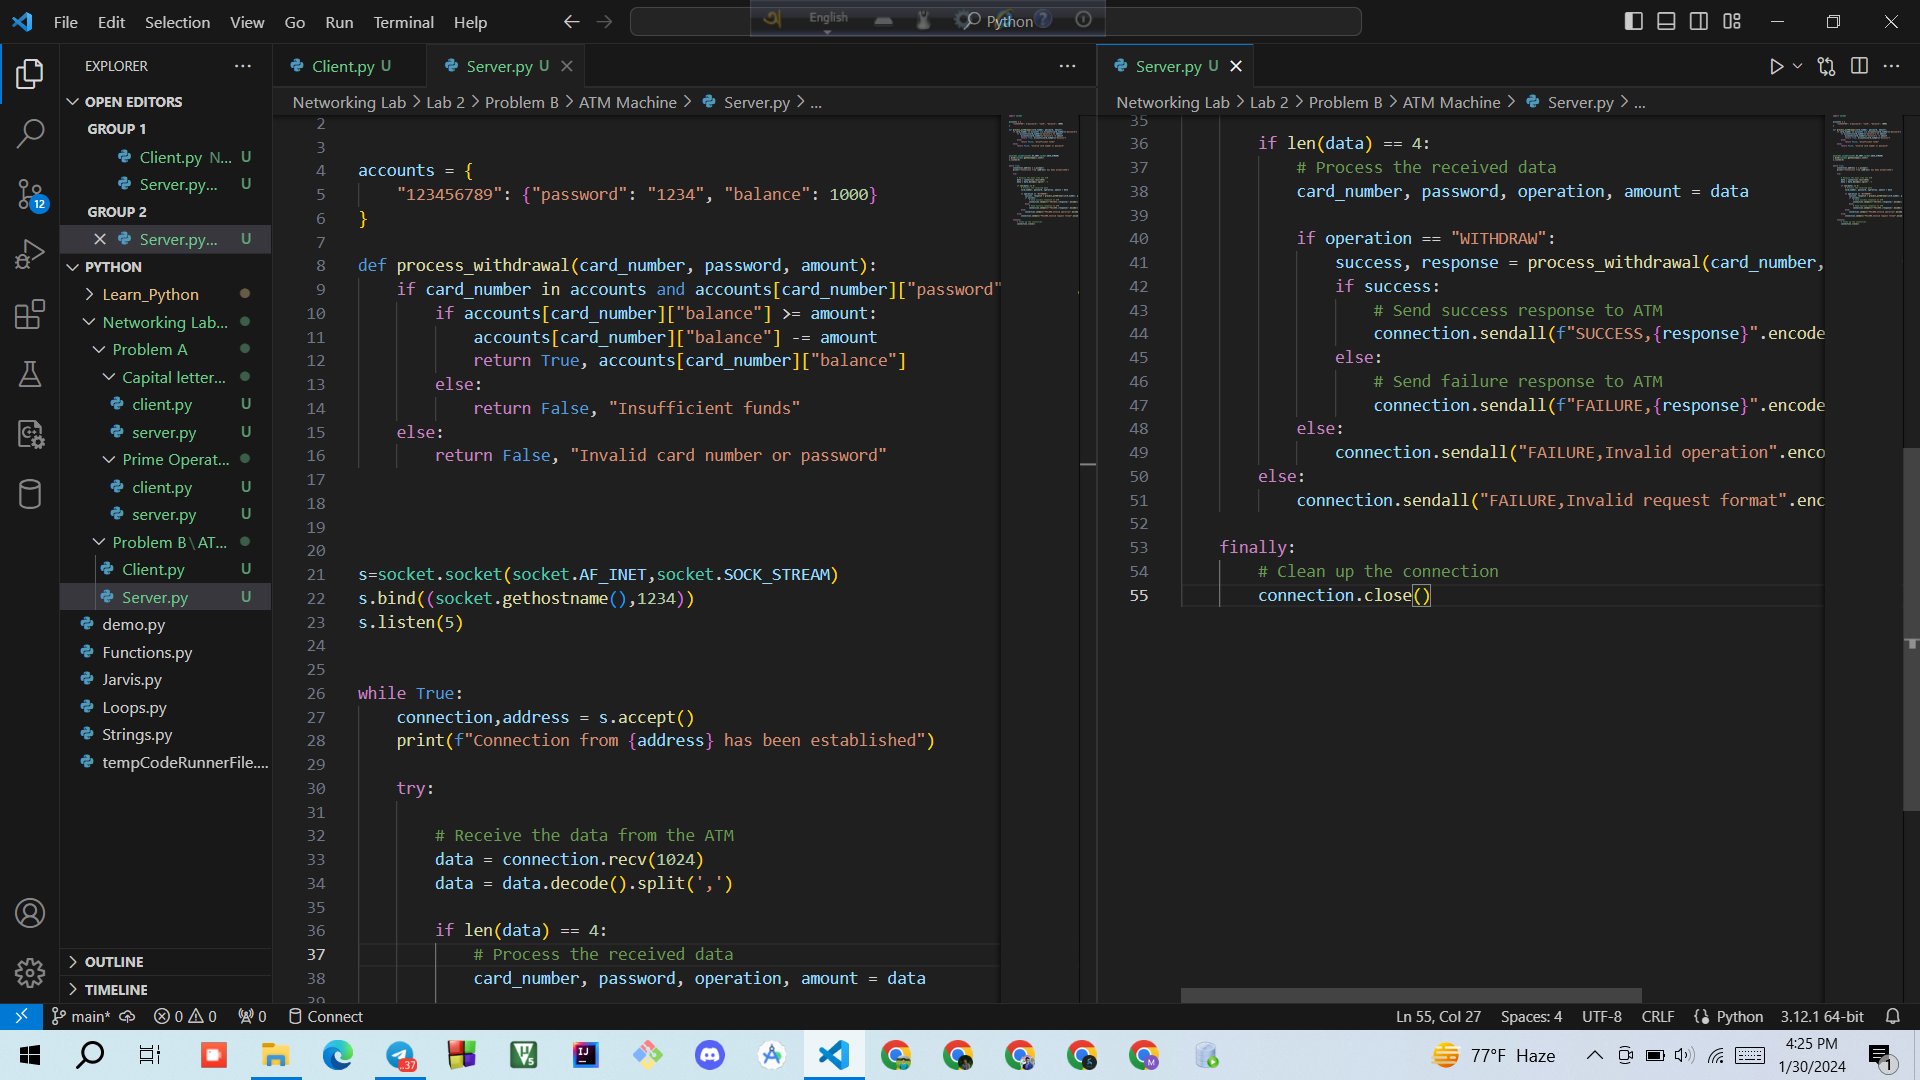
\includegraphics[width=0.8\textwidth]{atm.server.png}
        \caption{Server Side Code}
        \label{fig:2}
    \end{figure}
    
    \begin{figure}[H]
      \centering
      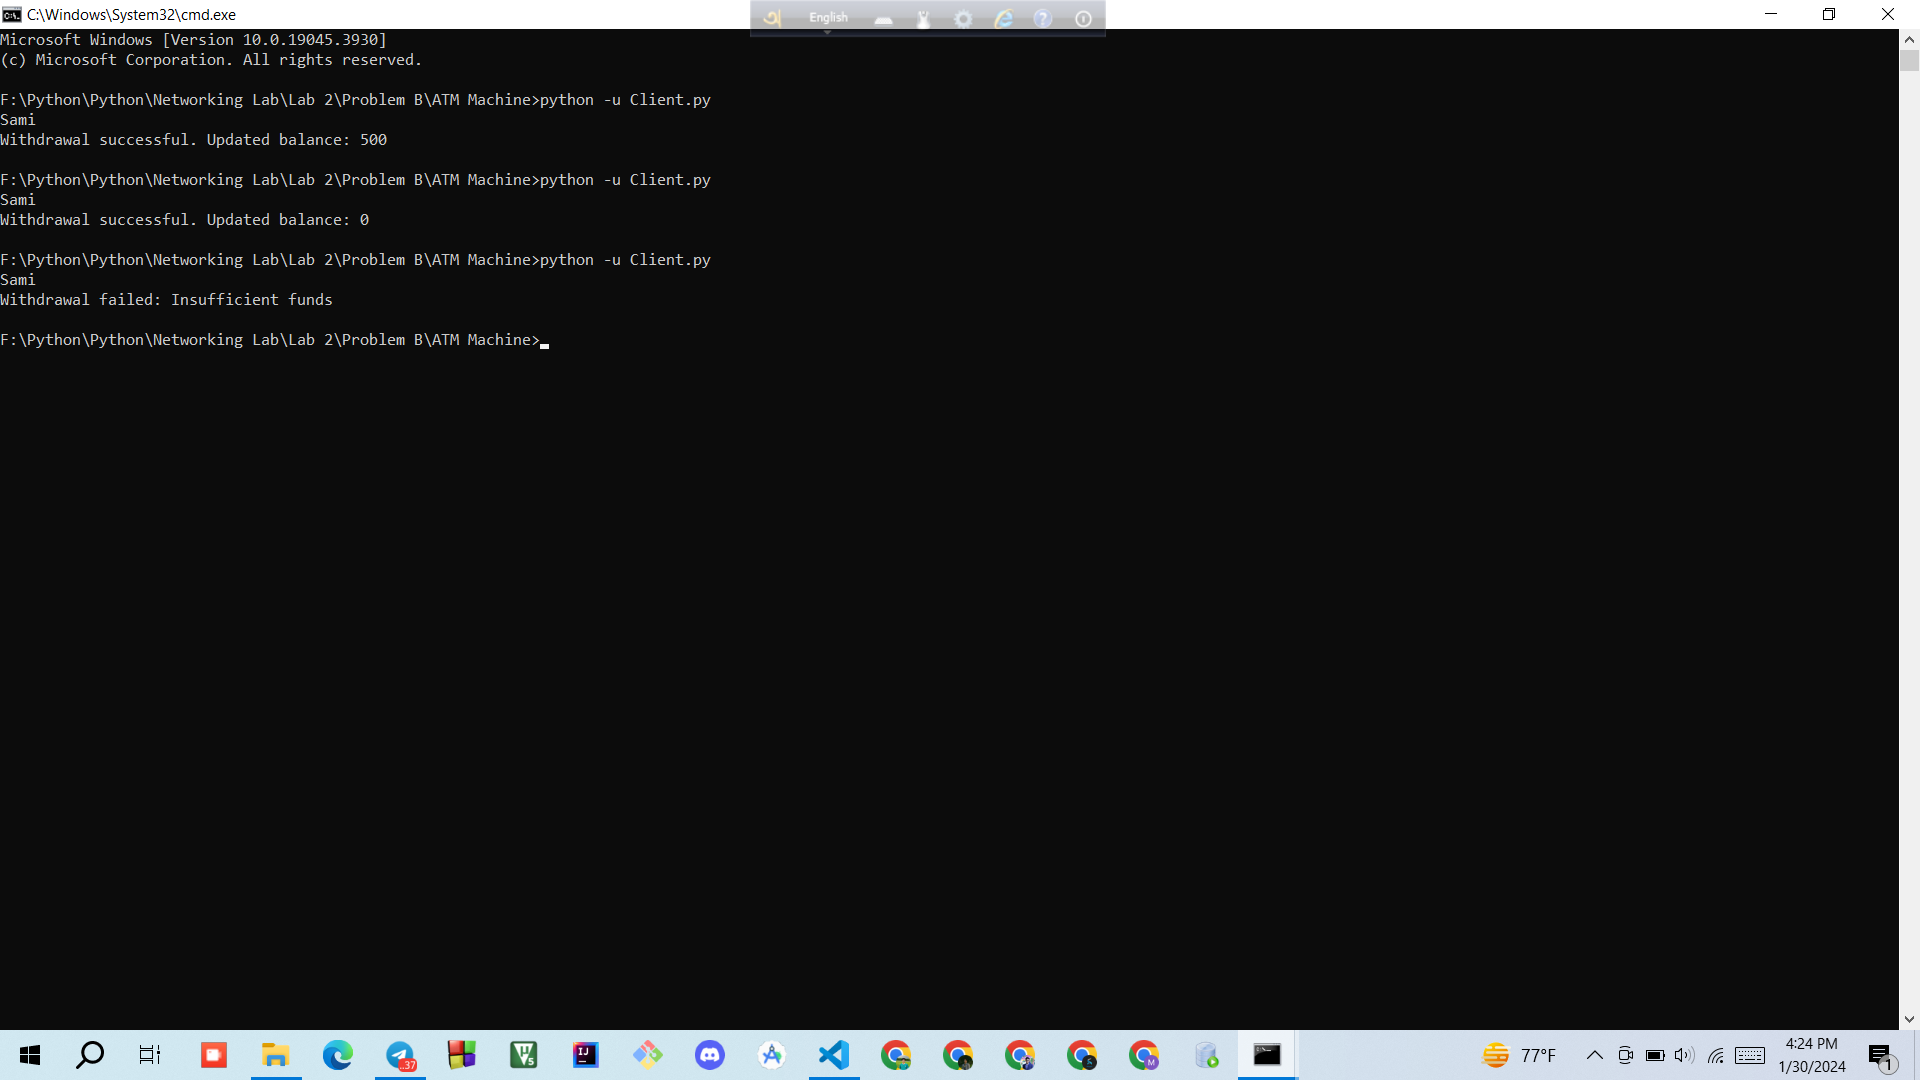
\includegraphics[width=0.8\textwidth]{atm_result.client.png}
      \caption{Client Side result}
      \label{fig:3}
    \end{figure}
    
    \begin{figure}[H]
      \centering
      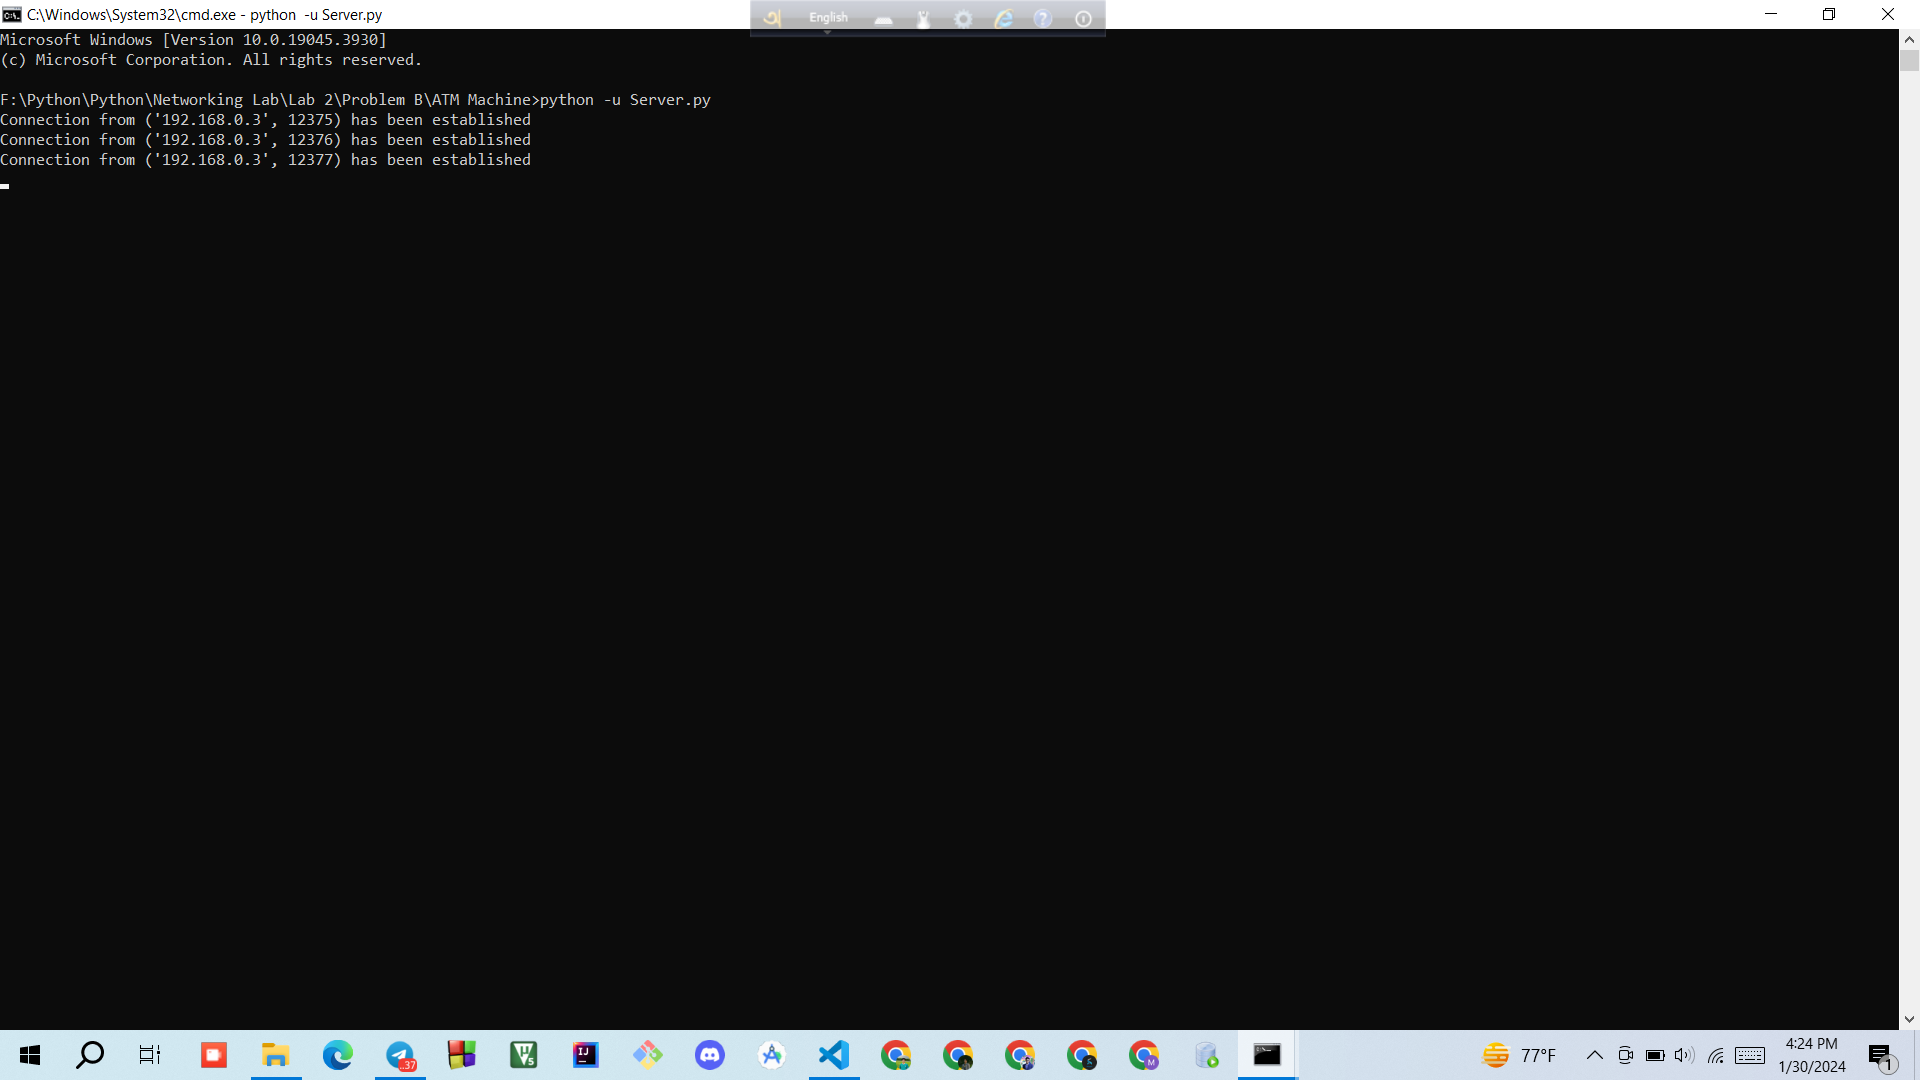
\includegraphics[width=0.8\textwidth]{atm_result.server.png}
      \caption{Server Side result}
      \label{fig:4}
    \end{figure}

\end{itemize}



\subsection{Error Handelling}


\begin{itemize}
    
    
    
    \begin{minted}[mathescape, linenos]{python}
    SERVER SIDE CODE
   
import socket

s = socket.socket(socket.AF_INET, socket.SOCK_STREAM)
s.bind((socket.gethostname(), 1234))
s.listen(5)
count=0
strr=""

while True:
    try:
        clientsocket, address = s.accept()
        print(f"Connection from {address} has been established")
      
        msgg= clientsocket.recv(1024)
        x=(msgg.decode())
        
        
       
        strr=strr+x
        print(strr)
        #if x>=3:
        clientsocket.sendall(strr.encode())
    
        #else:
        #    clientsocket.sendall("Error".encode())
            

        
    except Exception as e:
        print(f"Error: {e}")


    clientsocket.close()



\end{minted}


    \begin{minted}[mathescape, linenos]{python}
    CLIENT SIDE CODE
import socket
import random

# Socket creation and connection
s = socket.socket(socket.AF_INET, socket.SOCK_STREAM)
s.connect((socket.gethostname(), 1234))
count = 0

try:
    for x in range(1, 10):
        number = random.randint(0, 10)
        s.sendall(str(number).encode())
          
    #s.sendall("clear".encode())    
    response = s.recv(1024).decode() 
    for digit_char in response:
        digits = int(digit_char)
        if digits > 2:
            count += 1
    print(response)
    print("The Error is ", (100 - (count * 10)), "%")

finally:
    s.close()

\end{minted}
    \begin{figure}[H]
        \centering
        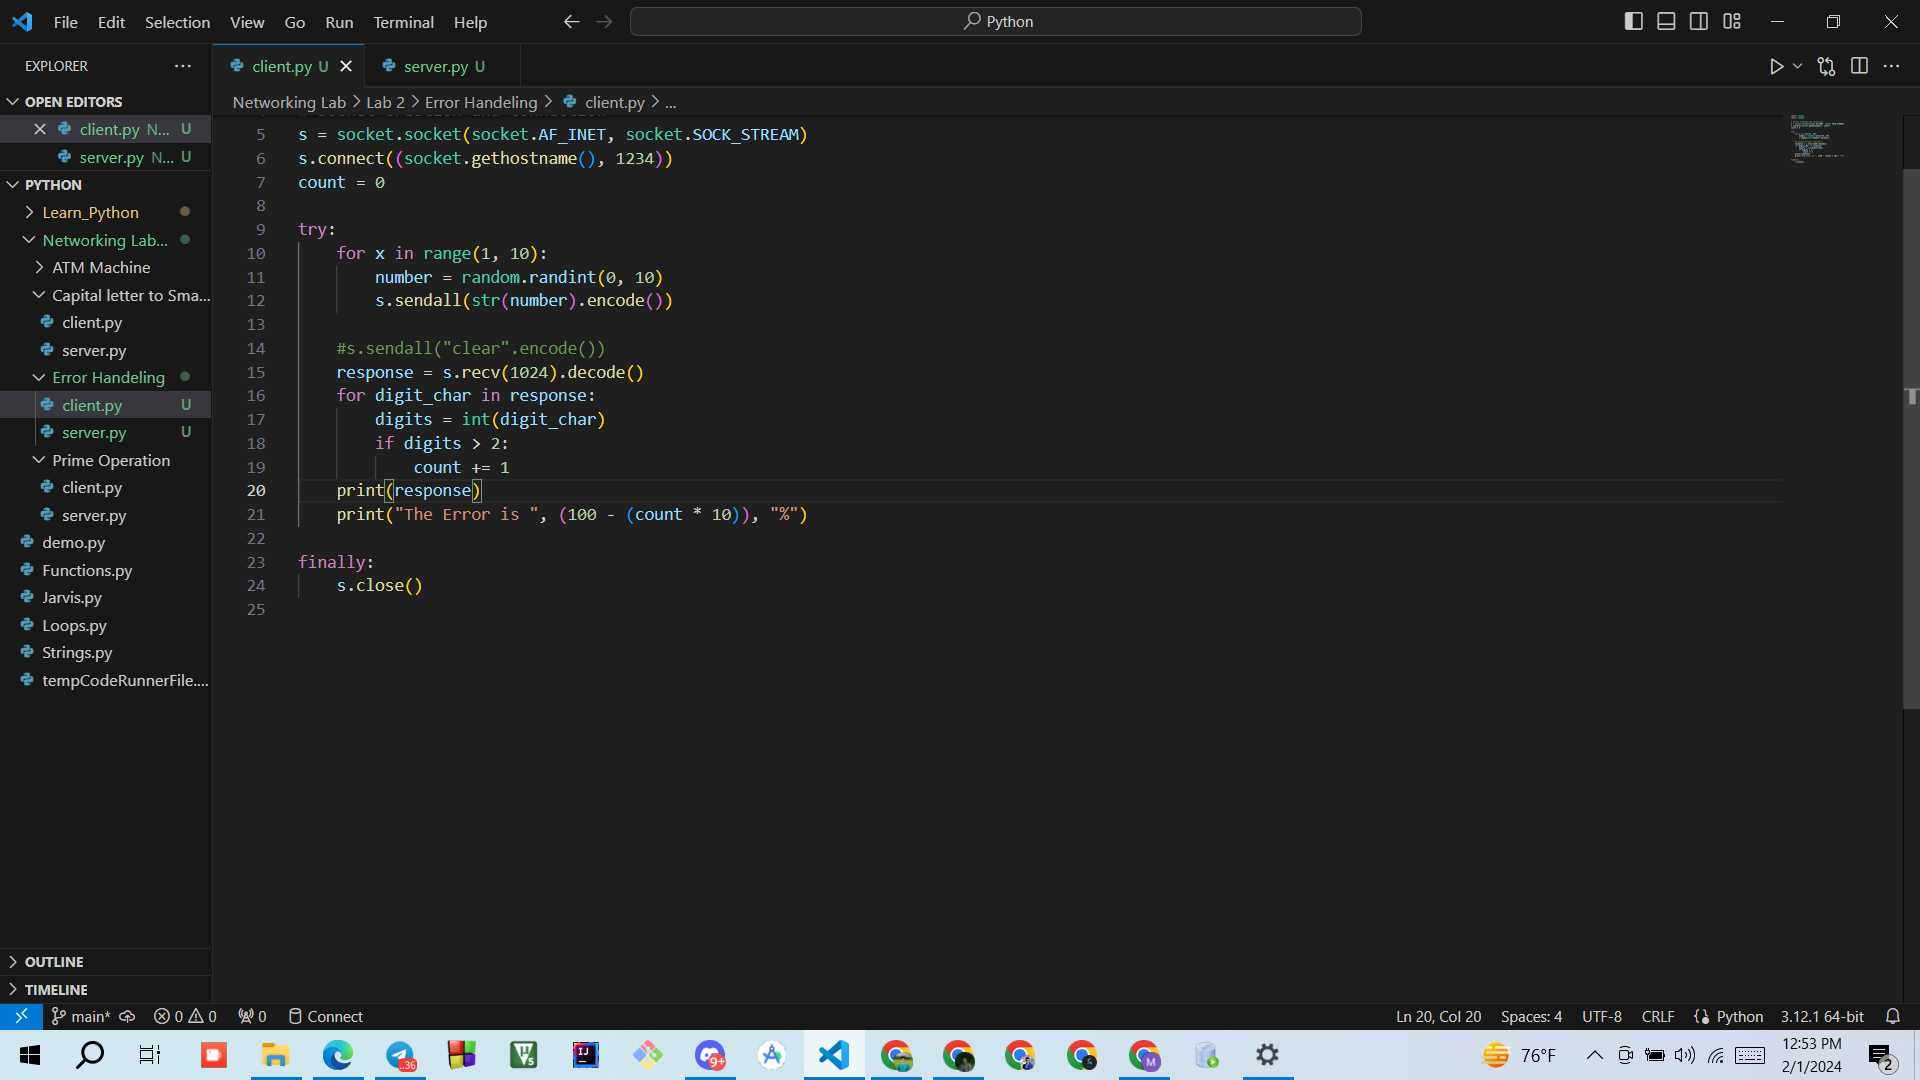
\includegraphics[width=0.8\textwidth]{Error_client.png}
        \caption{Client side code}
        \label{fig:1}
    \end{figure}
    
    \begin{figure}[H]
        \centering
        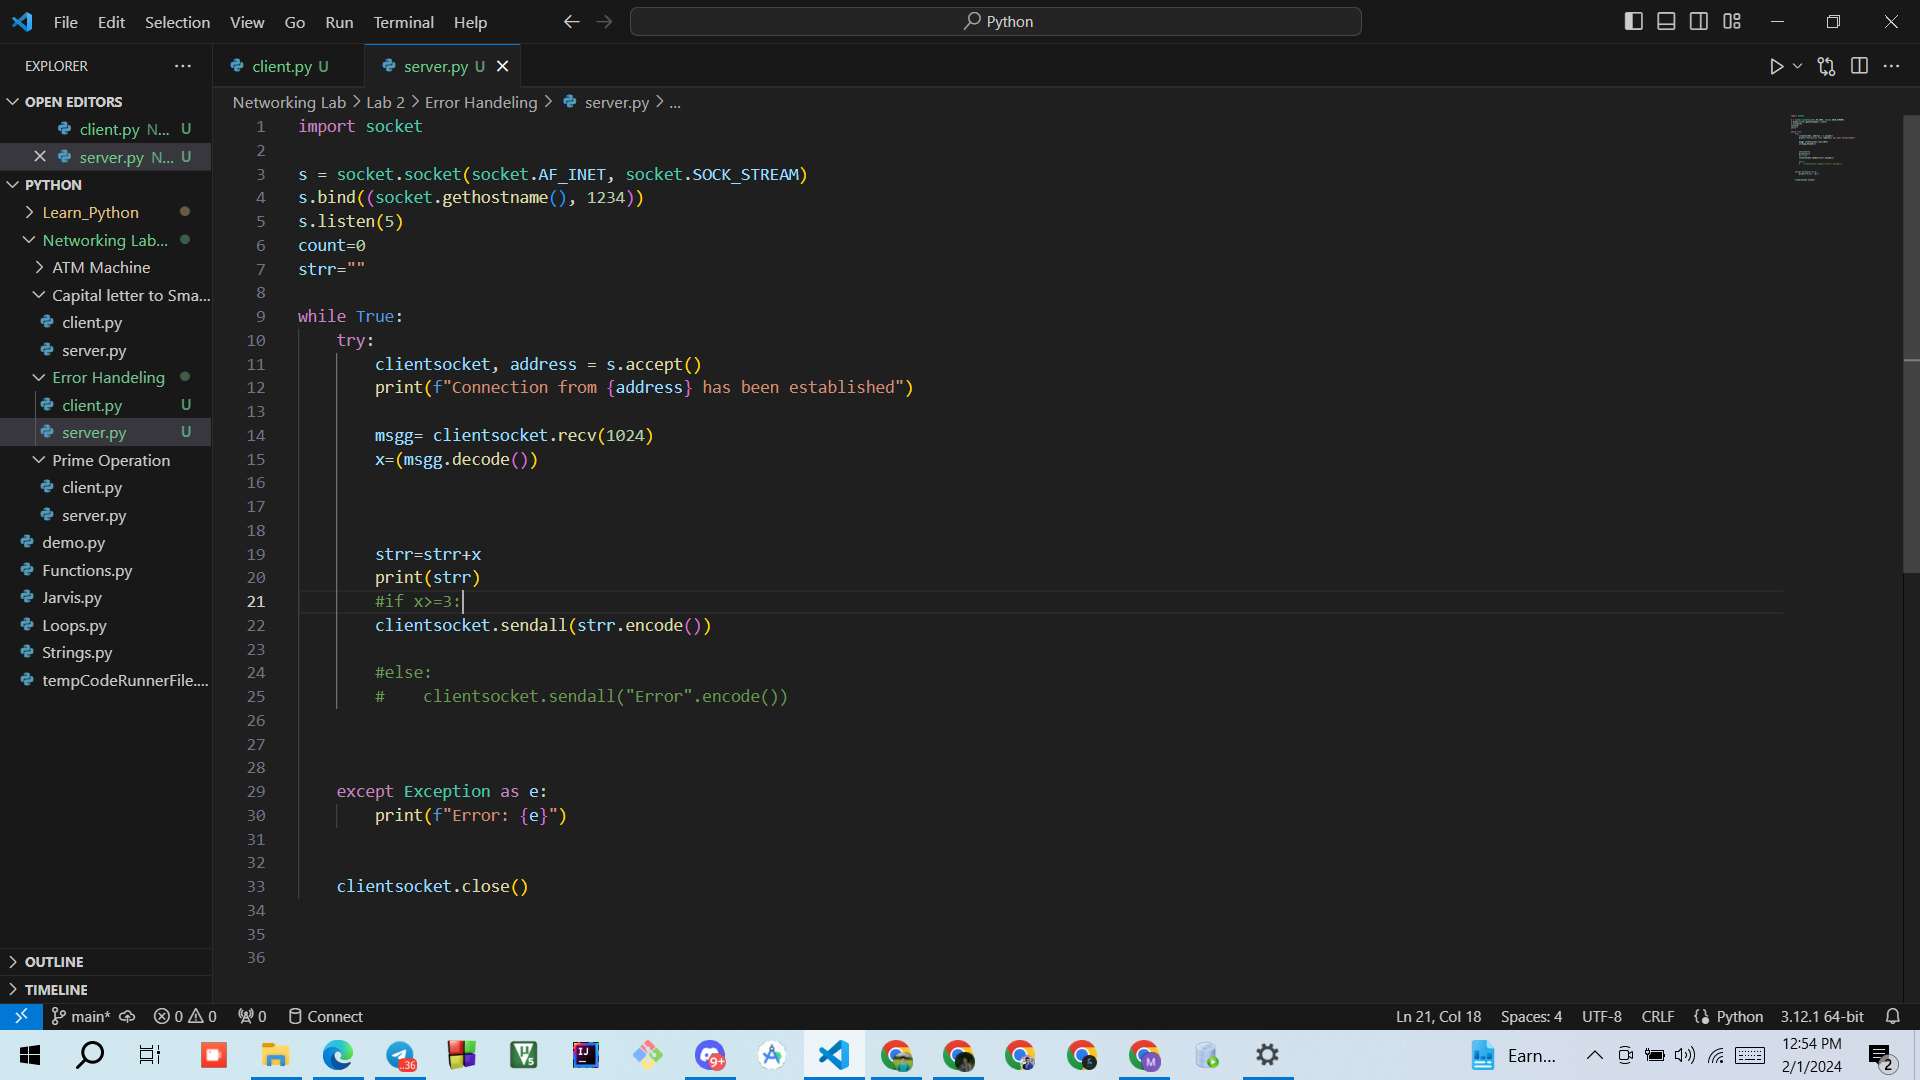
\includegraphics[width=0.8\textwidth]{Error_server.png}
        \caption{Server Side Code}
        \label{fig:2}
    \end{figure}
    
    \begin{figure}[H]
      \centering
      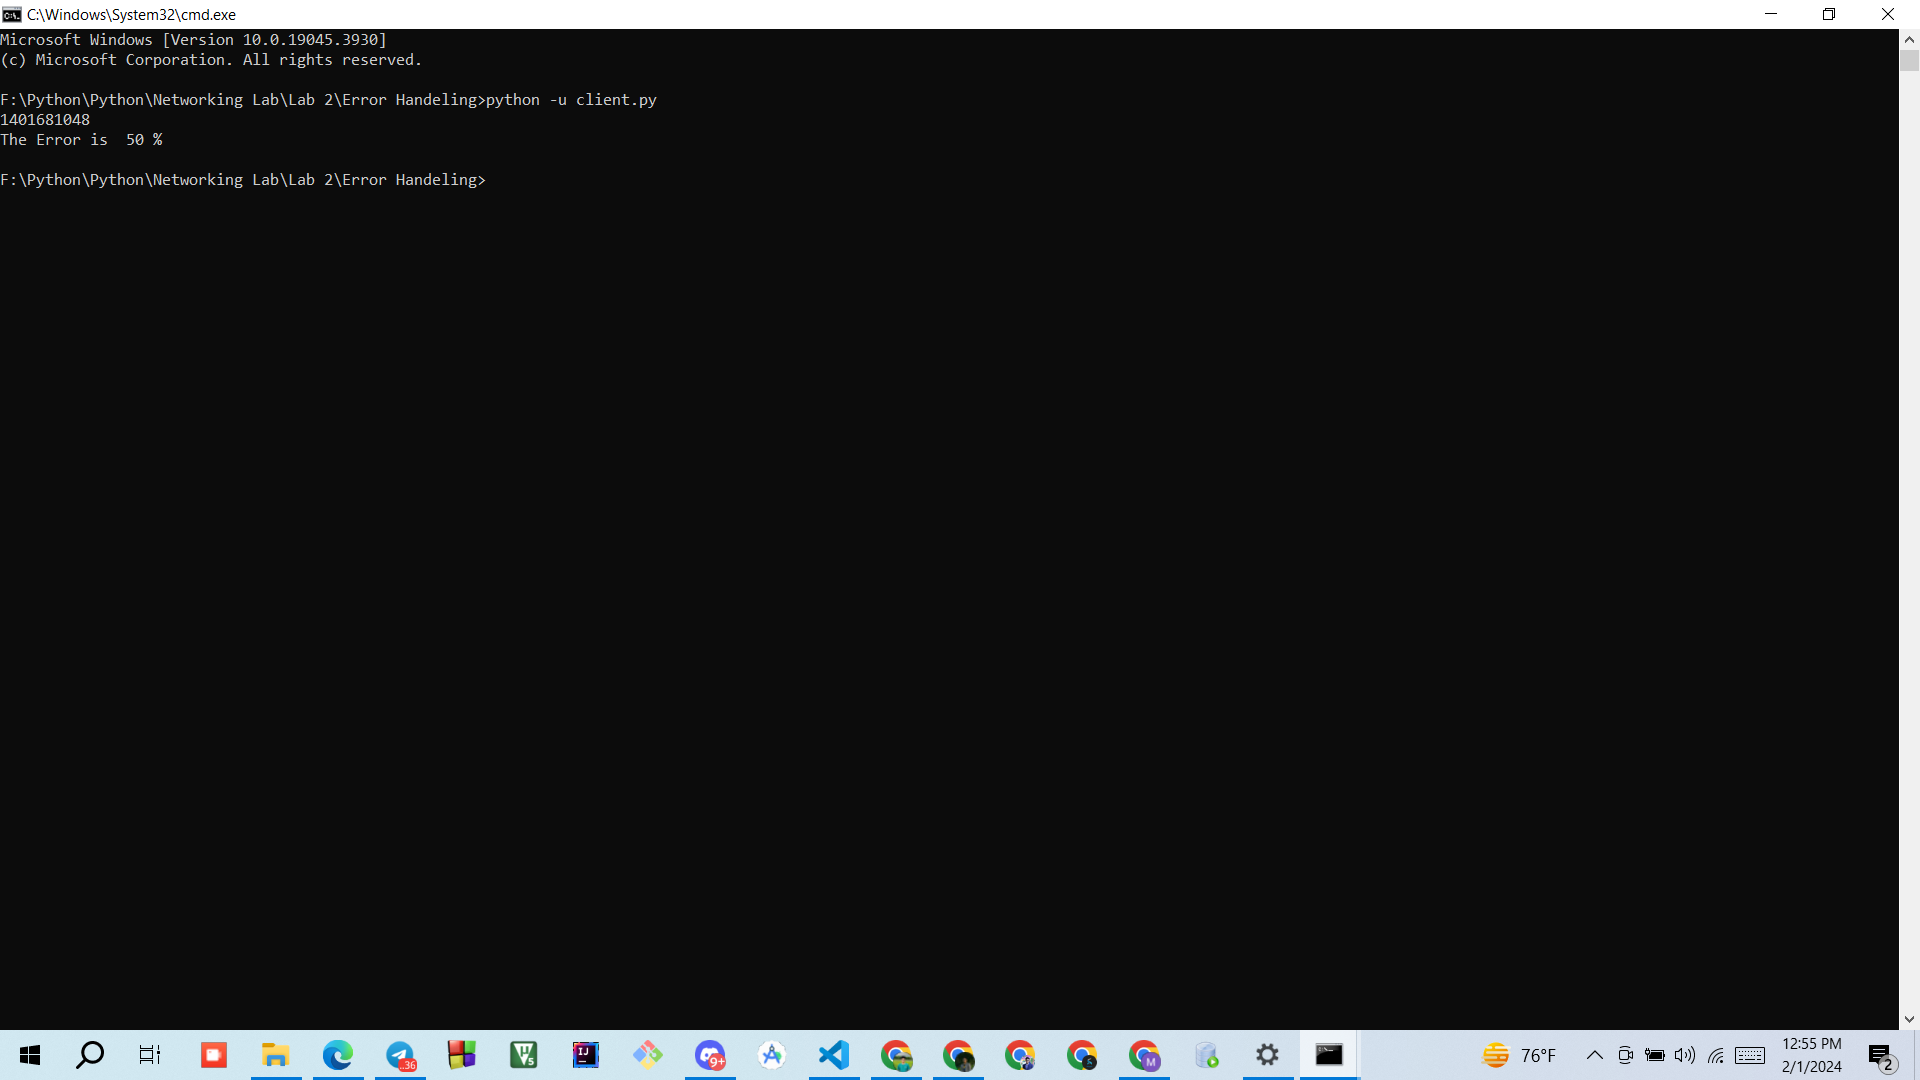
\includegraphics[width=0.8\textwidth]{Error_result_client.png}
      \caption{Client Side result}
      \label{fig:3}
    \end{figure}
    
    \begin{figure}[H]
      \centering
      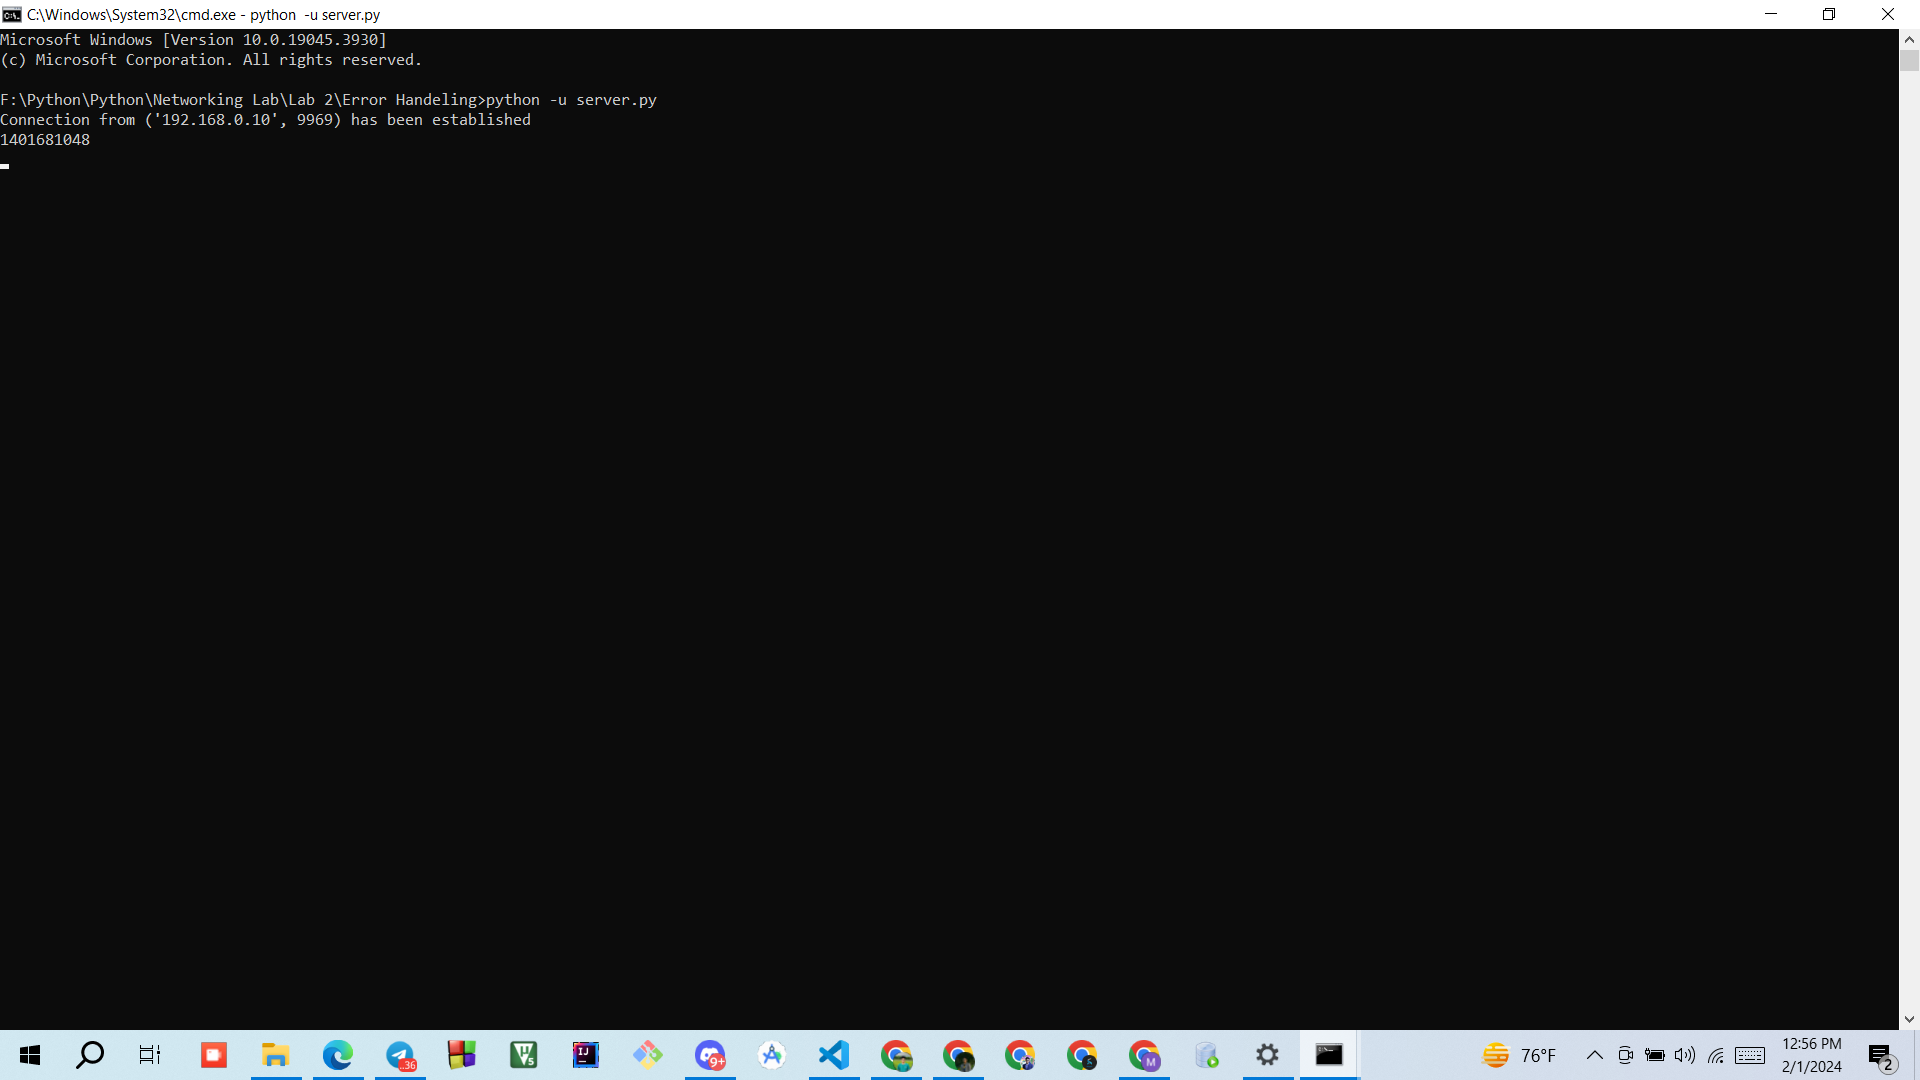
\includegraphics[width=0.8\textwidth]{Error_result_server.png}
      \caption{Server Side result}
      \label{fig:4}
    \end{figure}

\end{itemize}







\newpage
\section{Experience}
\begin{enumerate}
    \item We had to see some examples of how to use Server-Client package in Python.
    \item We had to compile both of them on two different terminals or tabs.
    \item We had to run the Server program first. Then run the Client program.
    \item Then we had to type messages in the Client Window which will be received and shown by the Server Window simultaneously.
    \item Then we had to type "Over" to end the program.
\end{enumerate}




\begin{thebibliography}{1}
  %\bibitem{book} Computer networking: a top-down approach 6th ed.
  \bibitem{geeksforgeeks} Socket Programming in Python: \url{https://www.geeksforgeeks.org/socket-programming-python/}
  \bibitem{realpython} Socket Programming in Python: \url{https://realpython.com/python-sockets/}
\end{thebibliography}

















\end{document}
